\documentclass[12pt,a4paper]{article}

% ===== 自定义模板 =====
\usepackage[UTF8]{ctex}
\usepackage{amsmath}
\usepackage{graphicx}
\usepackage{geometry}
\usepackage{titlesec}
\usepackage{titletoc}
\usepackage{fancyhdr}
\usepackage{float}
\usepackage{caption}
\usepackage{booktabs}
\usepackage{xcolor}
\usepackage{listings}
\usepackage{hyperref}

% 页面设置
\geometry{left=2.5cm, right=2.5cm, top=2.5cm, bottom=2.5cm}

% 章节标题格式
\titleformat{\section}{\Large\bfseries\color{blue!60!black}}{\thesection}{1em}{}
\titleformat{\subsection}{\large\bfseries\color{blue!50!black}}{\thesubsection}{1em}{}

% 代码块设置
\lstset{
    basicstyle=\ttfamily\small,
    backgroundcolor=\color{gray!10},
    frame=single,
    framesep=5pt,
    breaklines=true,
    showstringspaces=false,
    keywordstyle=\color{blue},
    commentstyle=\color{green!60!black},
    stringstyle=\color{red!70!black}
}

% 页眉页脚
\pagestyle{fancy}
\fancyhf{}
\fancyhead[L]{\small 系统开发工具基础}
\fancyhead[R]{\small 第二次实验报告}
\fancyfoot[C]{\thepage}
\renewcommand{\headrulewidth}{0.4pt}

% 图片路径
\graphicspath{{./}}

% 超链接设置
\hypersetup{
    colorlinks=true,
    linkcolor=blue!60!black,
    citecolor=blue!60!black,
    urlcolor=blue!80!black
}

\title{\vspace{3cm}\Huge\textbf{系统开发工具基础}\\[0.5cm]
\LARGE 第二次实验报告\\[1cm]
\Large 命令行环境 \quad 开发环境与工具}
\author{丁翊君 \quad 学号：25020007016}
\date{2026年8月31日}

\begin{document}

\maketitle
\thispagestyle{empty}
\newpage

\tableofcontents
\newpage

% ============================================================
\section{实验目的}
% ============================================================

本次实验是《系统开发工具基础》课程的第二次实验，授课内容包括命令行环境、开发环境与工具、Debugging and Profiling 三部分。目前已完成前三题，主题如下：

\begin{enumerate}
    \item \textbf{命令行环境：进程、信号与任务控制}：掌握 Shell 中后台任务的控制方法，理解进程信号与 \texttt{trap} 清理机制。
    \item \textbf{开发环境与工具}：使用 IDE 语言服务器完成语义重构，借助 ruff 做静态检查，并用 pytest 验证代码正确性。
    \item \textbf{Debugging}：使用调试器定位并修复归并排序中的索引缺陷。
\end{enumerate}

\section{实验环境}

\begin{table}[H]
\centering
\caption{实验环境配置（本地开发电脑）}
\begin{tabular}{|l|l|}
\hline
\textbf{项目} & \textbf{配置} \\
\hline
\multicolumn{2}{|l|}{\textbf{硬件信息}} \\
\hline
机型 & ASUSTeK TX Gaming FX608LP \\
\hline
处理器 & Intel Core Ultra 9 275HX（24 线程） \\
\hline
内存 & 32 GiB \\
\hline
显卡 & NVIDIA GeForce RTX 5070 Laptop GPU + Intel 核显 \\
\hline
磁盘 & 1.0 TB \\
\hline
\multicolumn{2}{|l|}{\textbf{软件信息}} \\
\hline
操作系统 & Ubuntu 26.04.1 LTS（64 位） \\
\hline
桌面环境 & GNOME 50（Wayland） \\
\hline
内核 & Linux 7.0.0-28-generic \\
\hline
Shell & GNU Bash 5.3.9 \\
\hline
Python & 3.14.4（.venv 虚拟环境） \\
\hline
git & 2.53.0 \\
\hline
pytest & 9.0.2 \\
\hline
ruff & 0.16.4 \\
\hline
XeTeX & TeX Live 2025 / Debian \\
\hline
IDE & PyCharm / VS Code（启用 Python 语言服务器） \\
\hline
\end{tabular}
\end{table}

% ============================================================
\section{课上实验内容}
% ============================================================

% ------------------------------------------------------------
\subsection{第5题：控制一个可清理的后台任务}

\subsubsection{题目要求}

将给定脚本保存为 \texttt{q05/worker.sh}，再完成任务控制。给定内容：

\begin{lstlisting}[language=bash]
#!/usr/bin/env bash
trap 'echo CLEAN_EXIT >> cleanup.log; exit 0' TERM INT
n=0
while true; do
    echo "$n"
    n=$((n+1))
    sleep 1
done
\end{lstlisting}

题目要求：

\begin{itemize}
    \item 赋予脚本执行权限，在前台启动，并把 stdout、stderr 分别写入 \texttt{stdout.log}、\texttt{stderr.log}。
    \item 使用 \texttt{Ctrl-Z} 挂起任务，再用 \texttt{bg} 让它在后台继续；使用 \texttt{jobs} 确认状态。
    \item 使用 \texttt{jobs -p} 或等价方式取得 PID，不得手工抄写 PID；发送 \texttt{SIGTERM} 并等待任务结束。
    \item 确认 \texttt{cleanup.log} 中出现 \texttt{CLEAN\_EXIT}，且任务已经退出；禁止使用 \texttt{kill -9}。
\end{itemize}

\subsubsection{执行过程与结果}

\begin{enumerate}
    \item 创建 \texttt{q05} 目录并编写 \texttt{worker.sh}，脚本通过 \texttt{trap} 捕获 \texttt{TERM}/\texttt{INT} 信号，收到信号时向 \texttt{cleanup.log} 写入 \texttt{CLEAN\_EXIT} 后退出；\texttt{chmod +x} 赋予执行权限。
    \item 前台启动脚本并把输出分离重定向：\texttt{./worker.sh > stdout.log 2> stderr.log}。
    \item 按 \texttt{Ctrl-Z} 将任务挂起（输出 \texttt{[1]+ 已停止}），再用 \texttt{bg} 放入后台继续运行。
    \item 用 \texttt{pid=\$(jobs -p \%1)} 取得任务 PID（不手工抄写），执行 \texttt{kill -TERM \$pid}。
    \item 查看 \texttt{cleanup.log}，出现 \texttt{CLEAN\_EXIT}，任务状态变为已完成。
\end{enumerate}

\begin{figure}[H]
\centering
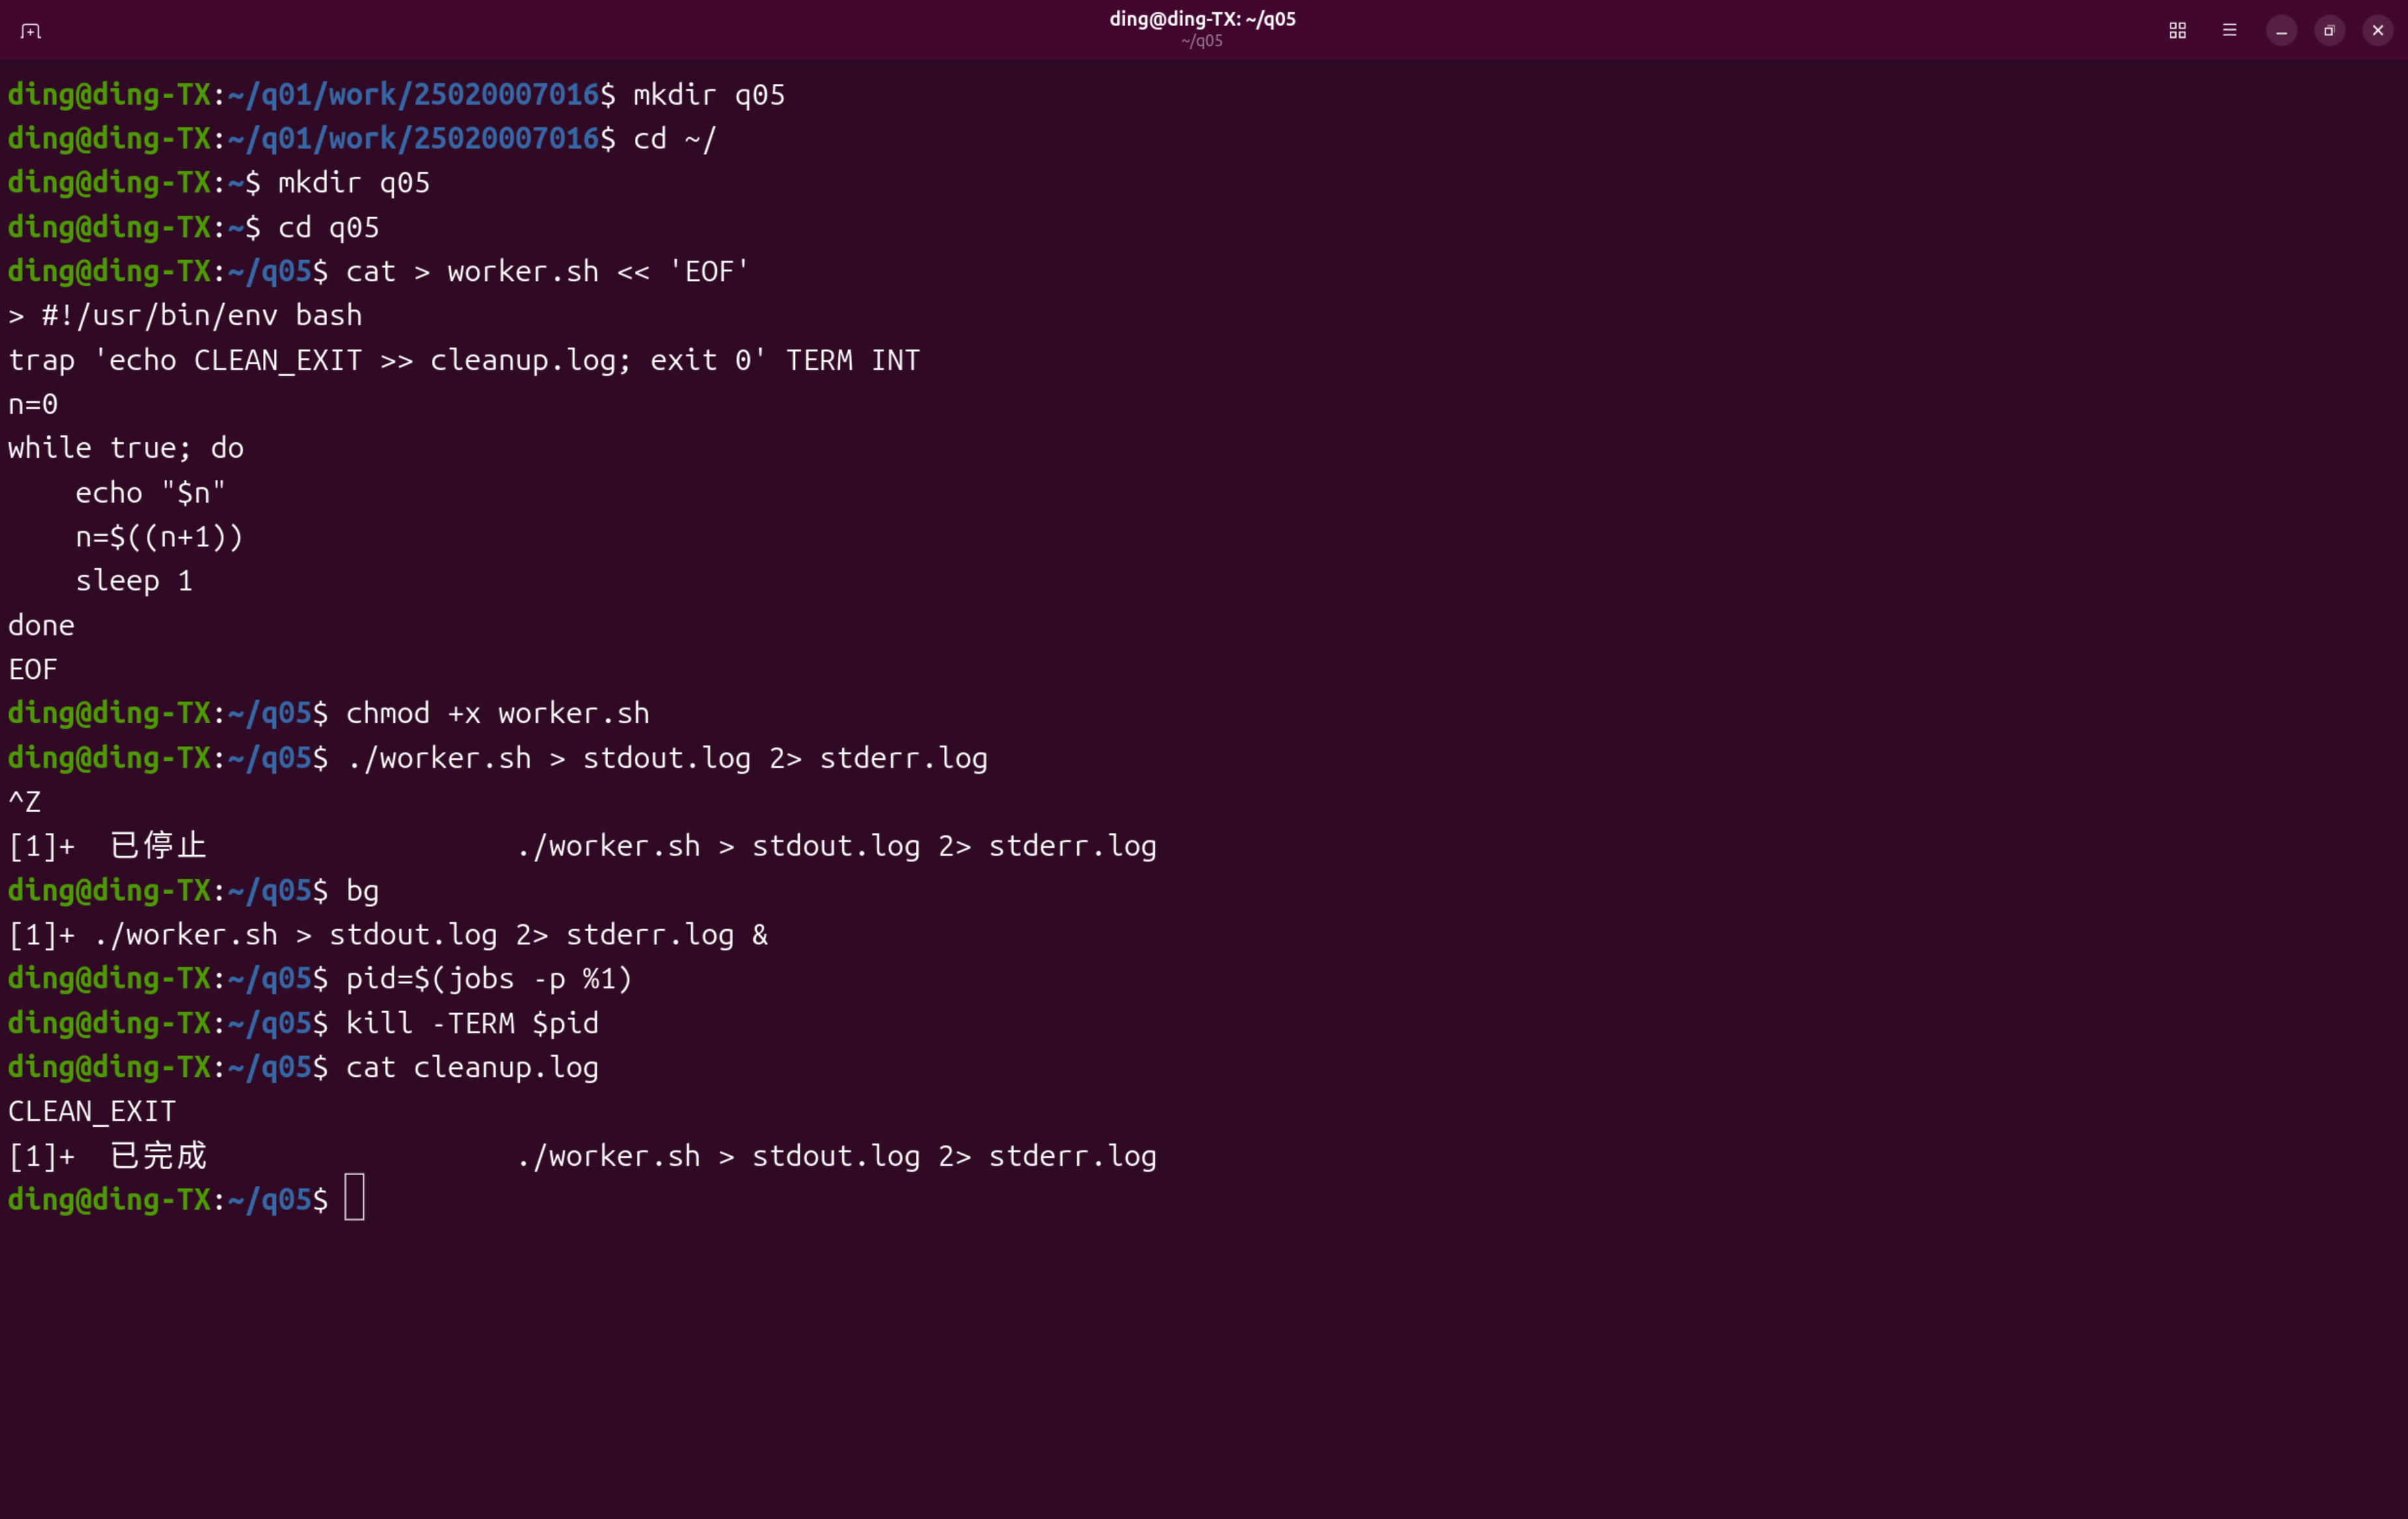
\includegraphics[width=0.95\textwidth]{q05_task_control.png}
\caption{第5题：后台任务控制完整过程（挂起、后台、取 PID、发送 SIGTERM）}
\end{figure}

\subsubsection{关键技术点}

\begin{enumerate}
    \item \textbf{信号与 \texttt{trap}}：\texttt{trap '命令' TERM INT} 在收到 \texttt{SIGTERM} 或 \texttt{SIGINT} 时执行指定命令，可以完成清理动作再退出；\texttt{kill -9}（SIGKILL）无法被捕获，会直接杀死进程、跳过清理。
    \item \textbf{任务控制}：\texttt{Ctrl-Z} 发送 \texttt{SIGTSTP} 挂起前台任务，\texttt{bg} 将其转为后台继续运行，\texttt{jobs} 查看任务列表与状态。
    \item \textbf{获取 PID}：\texttt{jobs -p \%1} 直接输出后台任务的 PID，避免人工抄写出错。
    \item \textbf{输出分离}：\texttt{> stdout.log 2> stderr.log} 分别重定向标准输出与标准错误，便于排查。
\end{enumerate}

% ------------------------------------------------------------
\subsection{第6题：语义重构与本地开发反馈}

\subsubsection{题目要求}

在 \texttt{q06} 中按照给定代码创建三个 Python 文件，并使用编辑器语言服务器完成一次语义重构。给定内容：

\begin{lstlisting}[language=Python]
# math_utils.py
def total_price(price: float, count: int) -> float:
    return price * count

# app.py
from math_utils import total_price
print(total_price(12.5, 4))

# test_math_utils.py
from math_utils import total_price
def test_total_price():
    assert total_price(12.5, 4) == 50.0
\end{lstlisting}

题目要求：

\begin{itemize}
    \item 在已配置好 Python、pytest 和 ruff 的课程环境中打开 \texttt{q06}，并启用 Python 语言服务器。
    \item 分别演示跳转到定义和查找引用。
    \item 使用“重命名符号”把 \texttt{total\_price} 改为 \texttt{calculate\_total}，保证定义和所有代码引用同步改变。
    \item 在 \texttt{app.py} 中临时加入未使用的 \texttt{import os}，用 ruff 发现并删除；最后运行 ruff 和 pytest 并保证通过。
\end{itemize}

\subsubsection{执行过程与结果}

\textbf{步骤1：创建三个 Python 文件。} 在 \texttt{q06} 下用 here-doc 写入 \texttt{math\_utils.py}、\texttt{app.py}、\texttt{test\_math\_utils.py}。

\begin{figure}[H]
\centering
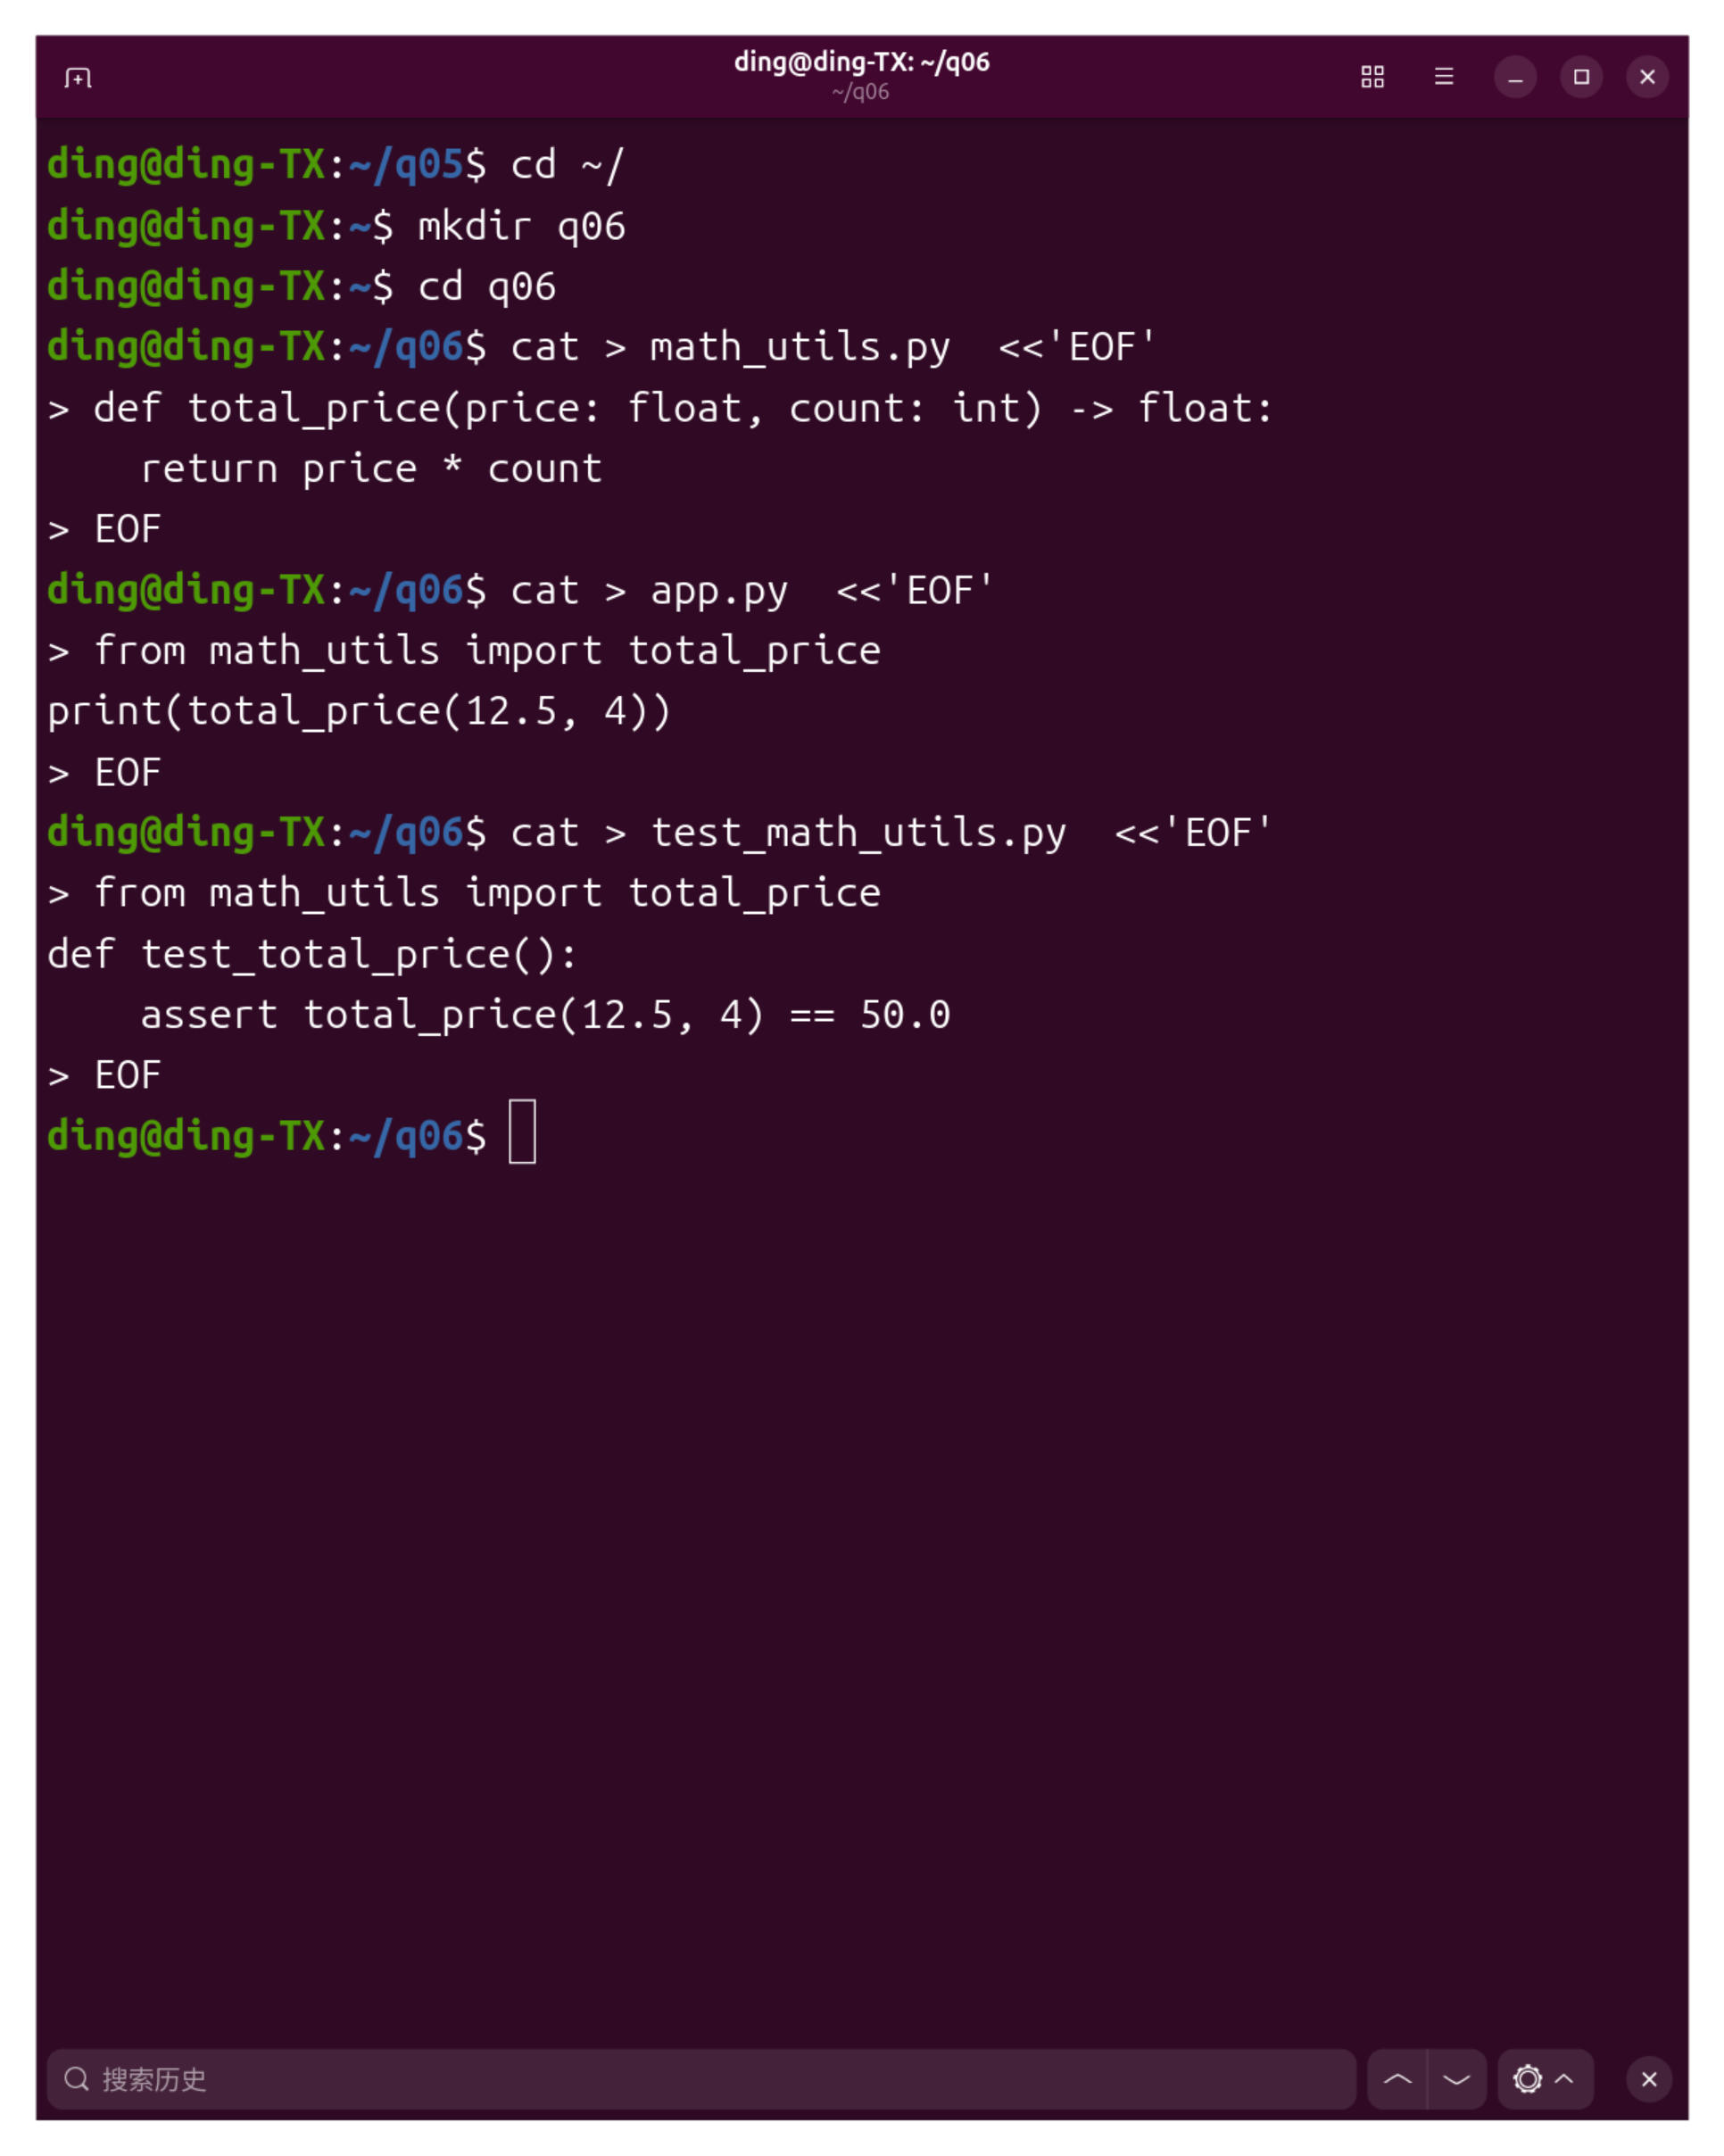
\includegraphics[width=0.9\textwidth]{q06_create_files.png}
\caption{第6题步骤1：创建三个 Python 文件}
\end{figure}

\textbf{步骤2：语言服务器跳转与重命名。} 在 PyCharm 中启用 Python 语言服务器，演示跳转到定义与查找引用；随后使用“重命名符号”把模块 \texttt{math\_utils} 重命名为 \texttt{calculate\_total}，\texttt{app.py} 与 \texttt{test\_math\_utils.py} 中的 import 引用全部同步更新。

\begin{figure}[H]
\centering
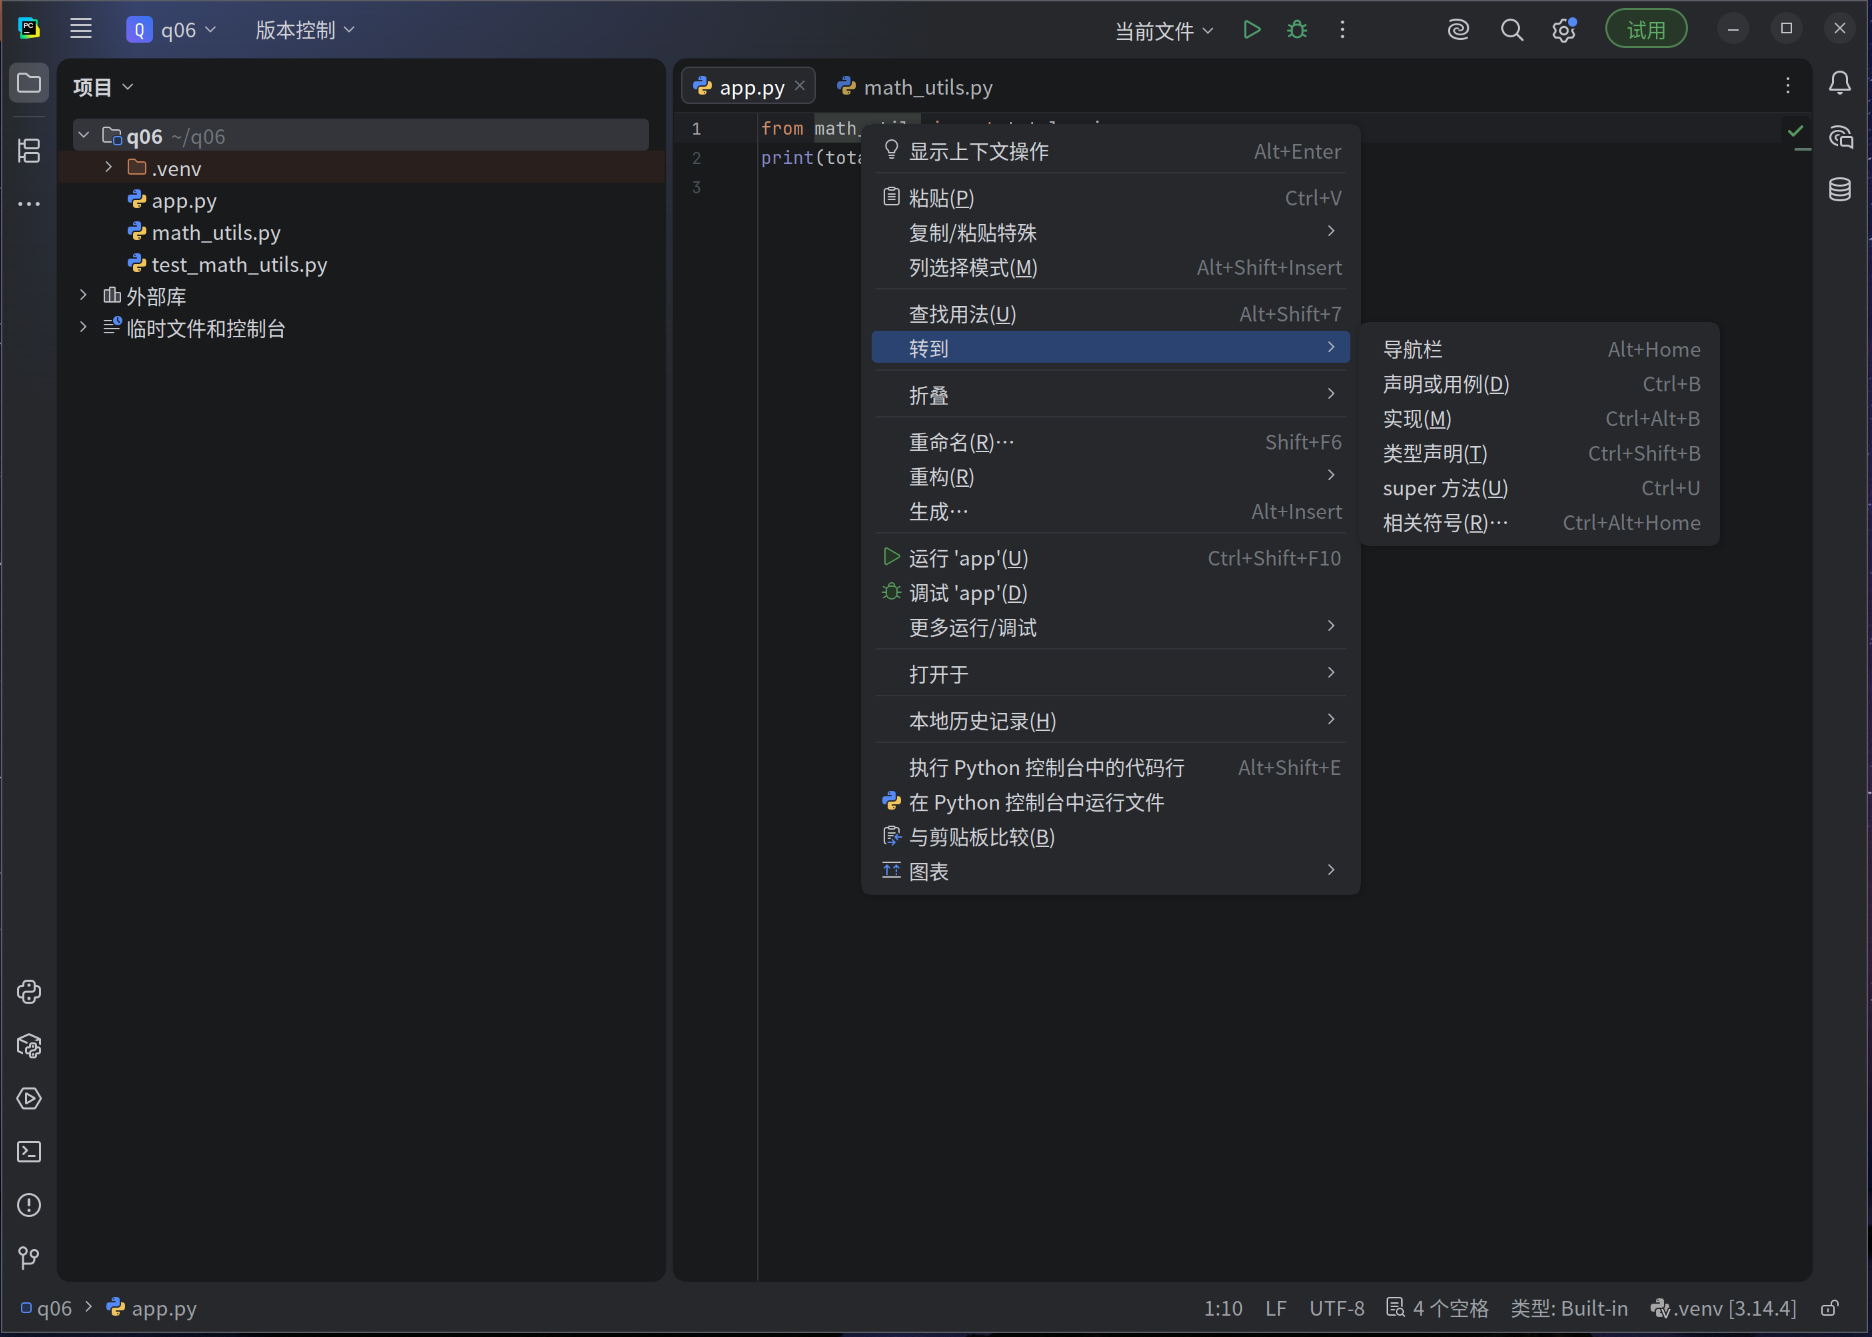
\includegraphics[width=0.9\textwidth]{q06_jump_to_def.png}
\caption{第6题步骤2：语言服务器跳转到定义 / 查找引用}
\end{figure}

\begin{figure}[H]
\centering
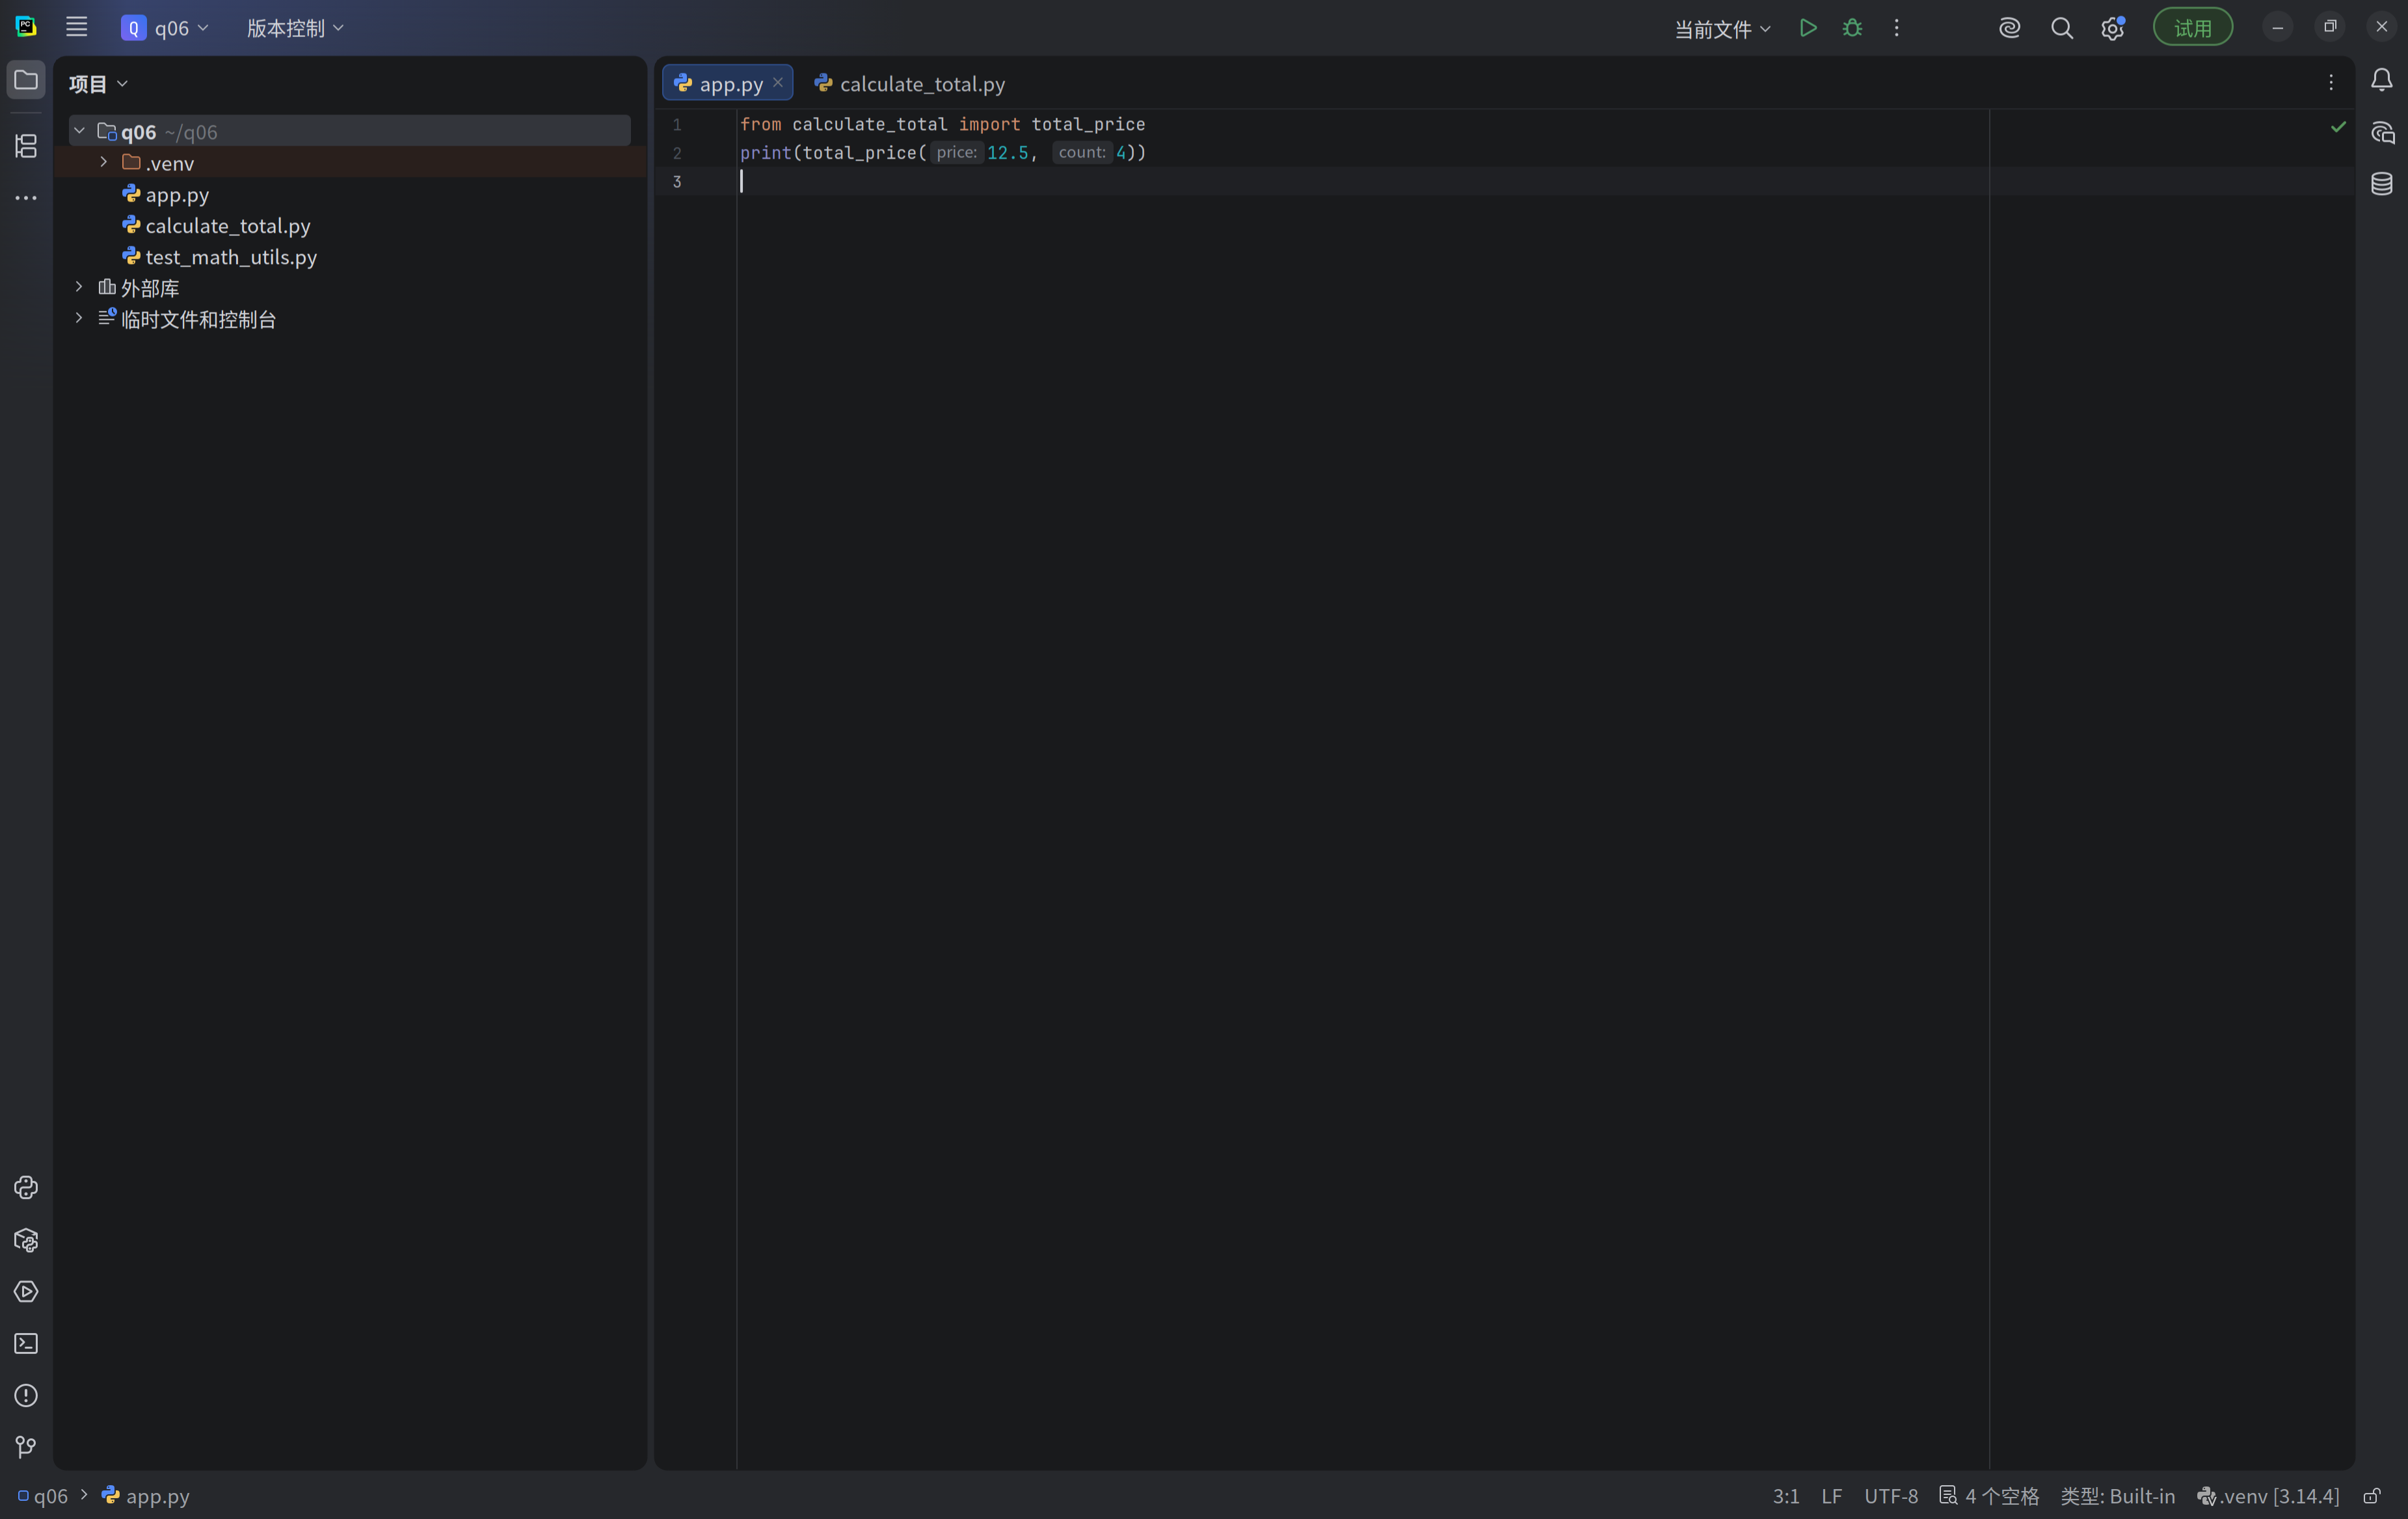
\includegraphics[width=0.9\textwidth]{q06_rename_symbol.png}
\caption{第6题步骤3：重命名符号为 calculate\_total（引用同步更新）}
\end{figure}

\textbf{步骤4：ruff 静态检查。} 在 \texttt{app.py} 临时加入未使用的 \texttt{import os}，安装 ruff 后执行 \texttt{ruff check}，报告 \texttt{I001}（导入块未排序/未格式化）与 \texttt{F401}（\texttt{os} 已导入但未使用），按提示删除该 import。

\begin{figure}[H]
\centering
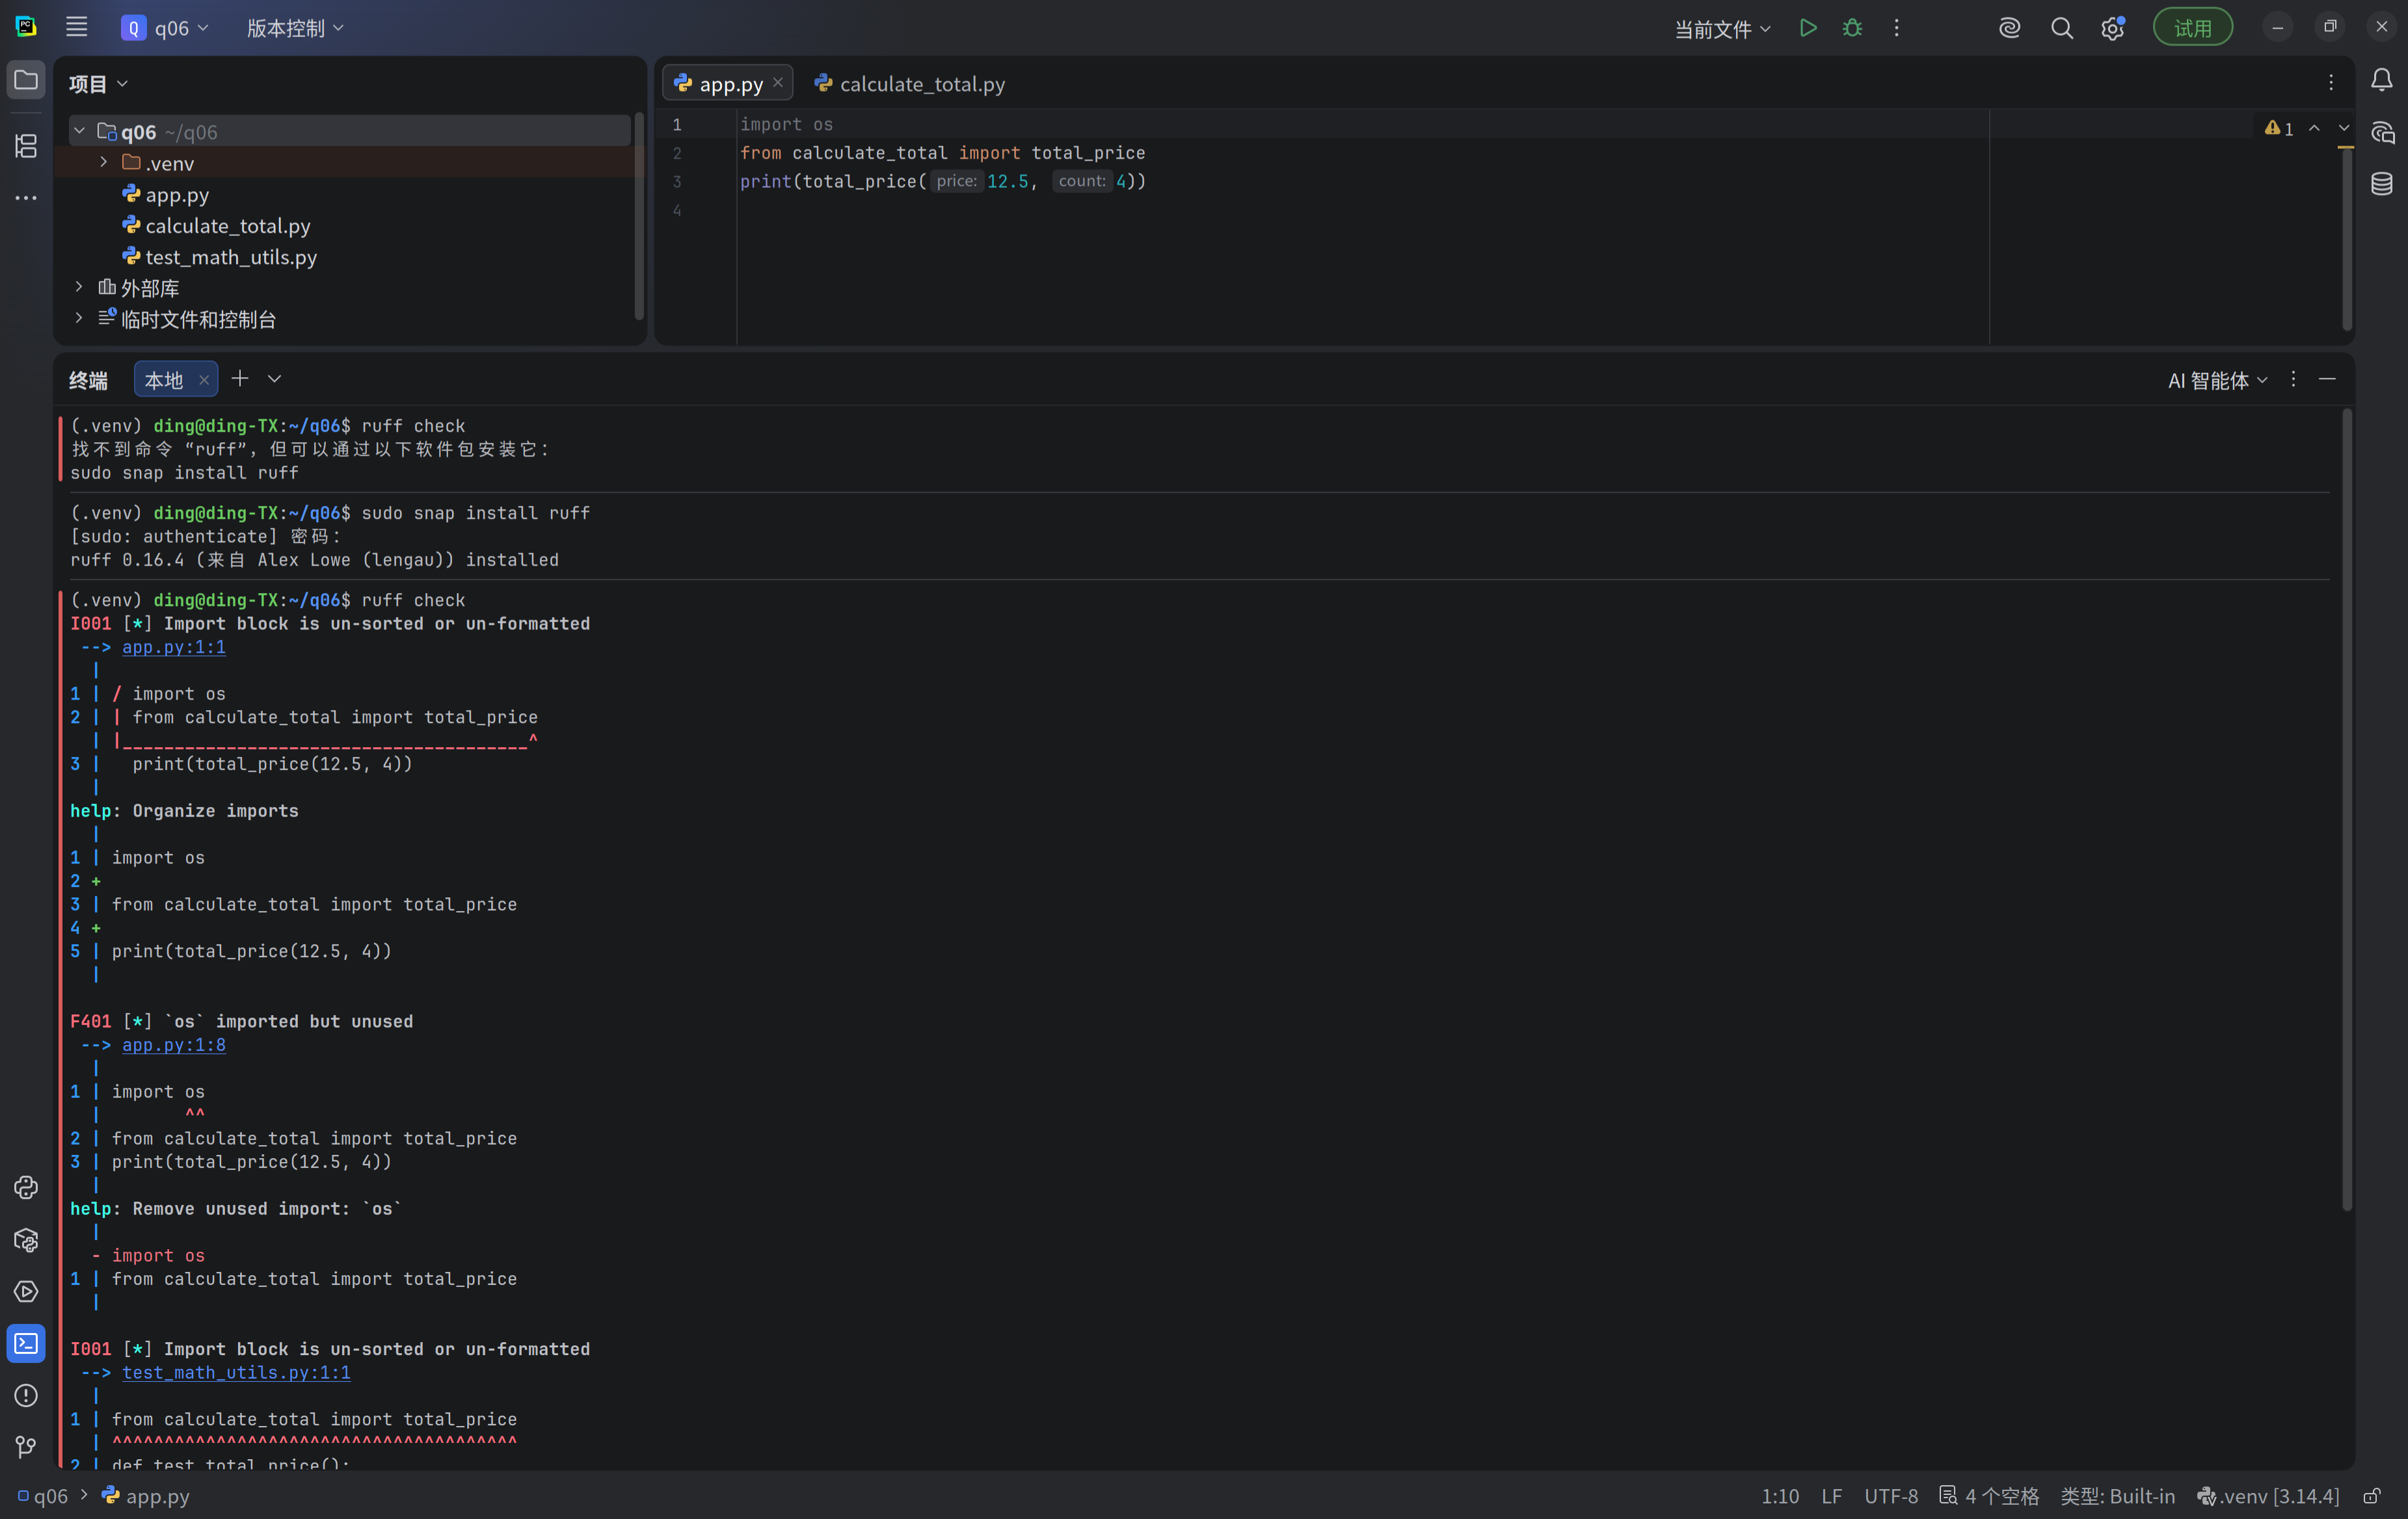
\includegraphics[width=0.9\textwidth]{q06_ruff_check.png}
\caption{第6题步骤4：ruff 发现未使用 import os}
\end{figure}

\textbf{步骤5：运行 pytest。} 安装 pytest 依赖后执行 \texttt{pytest}，收集到 1 个测试用例，\texttt{test\_math\_utils.py} 通过（1 passed in 0.01s）。

\begin{figure}[H]
\centering
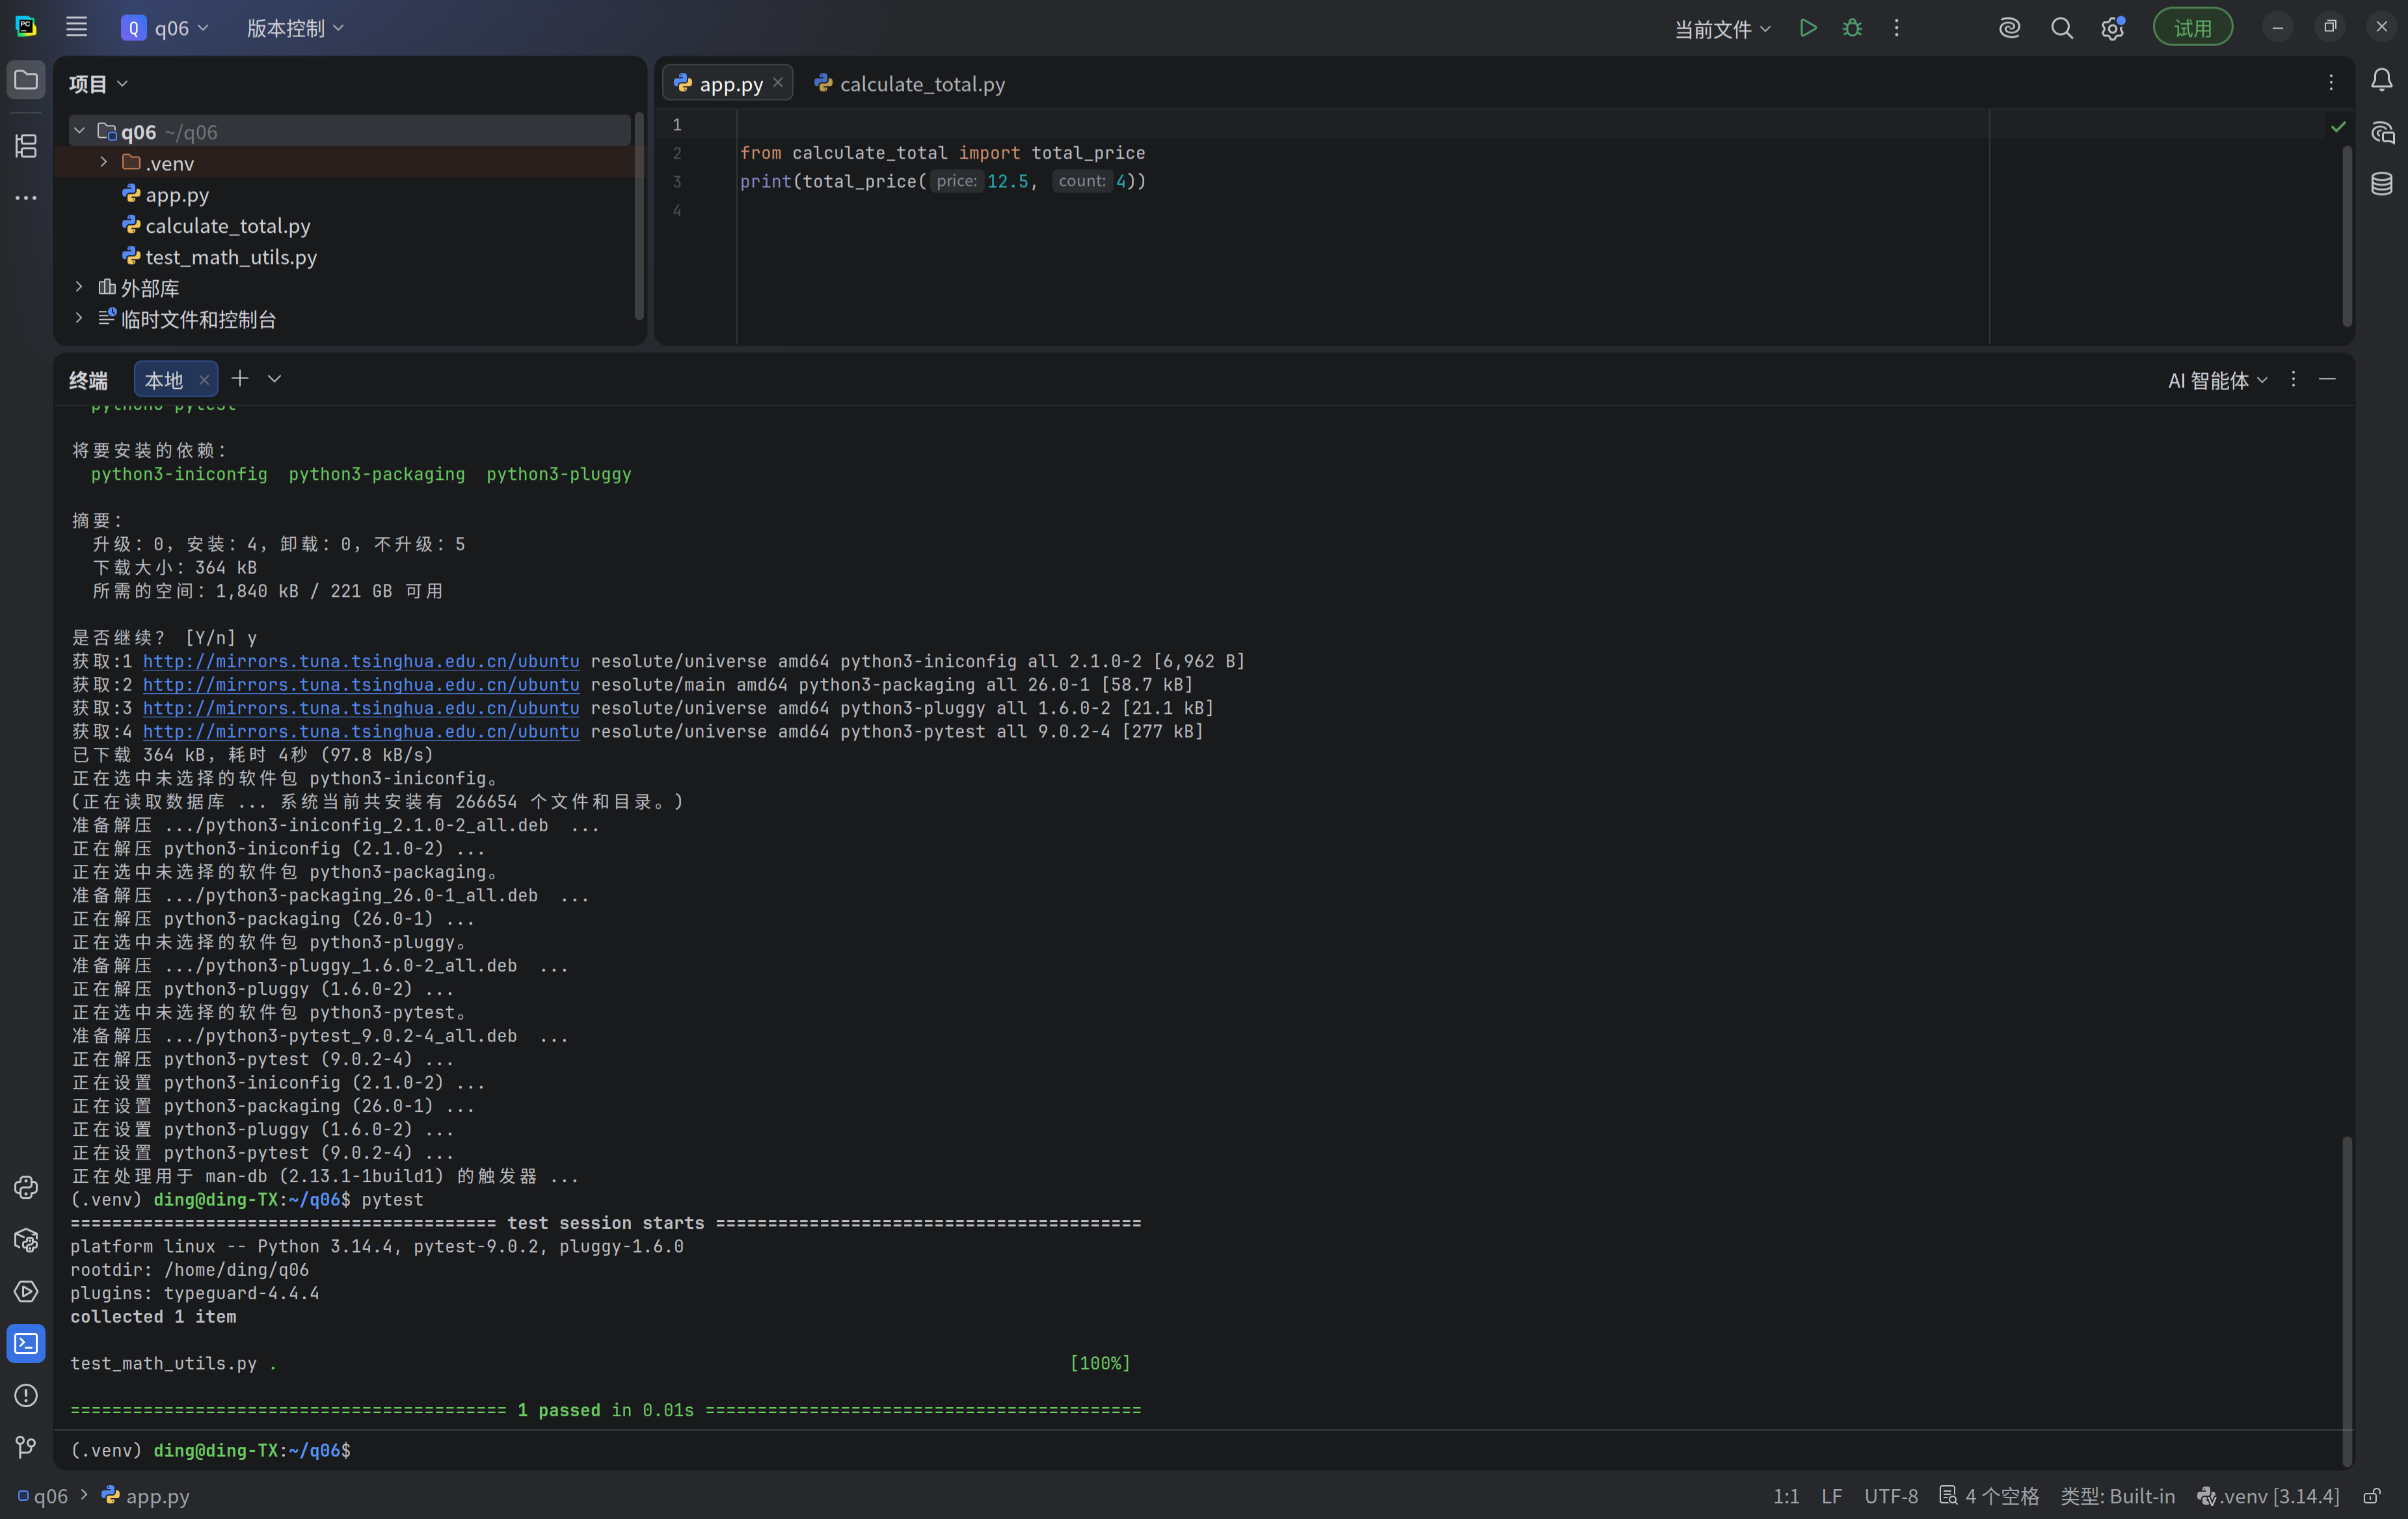
\includegraphics[width=0.9\textwidth]{q06_pytest.png}
\caption{第6题步骤5：pytest 单元测试通过}
\end{figure}

\subsubsection{关键技术点}

\begin{enumerate}
    \item \textbf{Python 语言服务器}：IDE 通过语言服务器获得跳转、引用、重命名等语义能力，而不是靠字符串匹配。
    \item \textbf{重命名符号}：一次重命名同时更新定义与所有引用，避免手改遗漏造成不一致。
    \item \textbf{ruff}：静态检查工具，\texttt{F401} 检查“导入但未使用”，\texttt{I001} 检查导入块排序与格式，可自动修复。
    \item \textbf{pytest}：以 \texttt{test\_} 前缀自动收集测试函数，断言不通过时给出失败信息，便于回归验证。
\end{enumerate}

% ------------------------------------------------------------
\subsection{第7题：用调试器定位归并排序缺陷}

\subsubsection{题目要求}

将下列存在缺陷的归并排序代码保存为 \texttt{q07/merge\_sort.py}，再使用调试器定位并修复。给定内容：

\begin{lstlisting}[language=Python]
def merge(left, right):
    result = []
    i = j = 0
    while i < len(left) and j < len(right):
        if left[i] <= right[j]:
            result.append(left[i]); i += 1
        else:
            result.append(right[i]); j += 1   # 此处存在缺陷
    return result + left[i:] + right[j:]

def merge_sort(a):
    if len(a) <= 1: return a
    m = len(a) // 2
    return merge(merge_sort(a[:m]), merge_sort(a[m:]))
print(merge_sort([3, 1, 4, 1, 5, 9, 2, 6]))
\end{lstlisting}

题目要求：

\begin{itemize}
    \item 先运行给定输入，确认结果错误或出现异常。
    \item 使用 pdb、IDE debugger 或等价调试器，在 \texttt{merge} 中设置断点并观察 \texttt{i}、\texttt{j}、\texttt{left[i]}、\texttt{right[j]}。
    \item 完成最小修复，不得用 \texttt{sorted} 替换归并排序。
    \item 使用 pytest 增加两个测试：给定输入和含重复元素的列表；保证测试通过。
\end{itemize}

\subsubsection{执行过程与结果}

\textbf{步骤1：创建脚本并运行。} 在 \texttt{q07} 下创建 \texttt{merge\_sort.py}（含缺陷代码），先运行确认结果异常。

\begin{figure}[H]
\centering
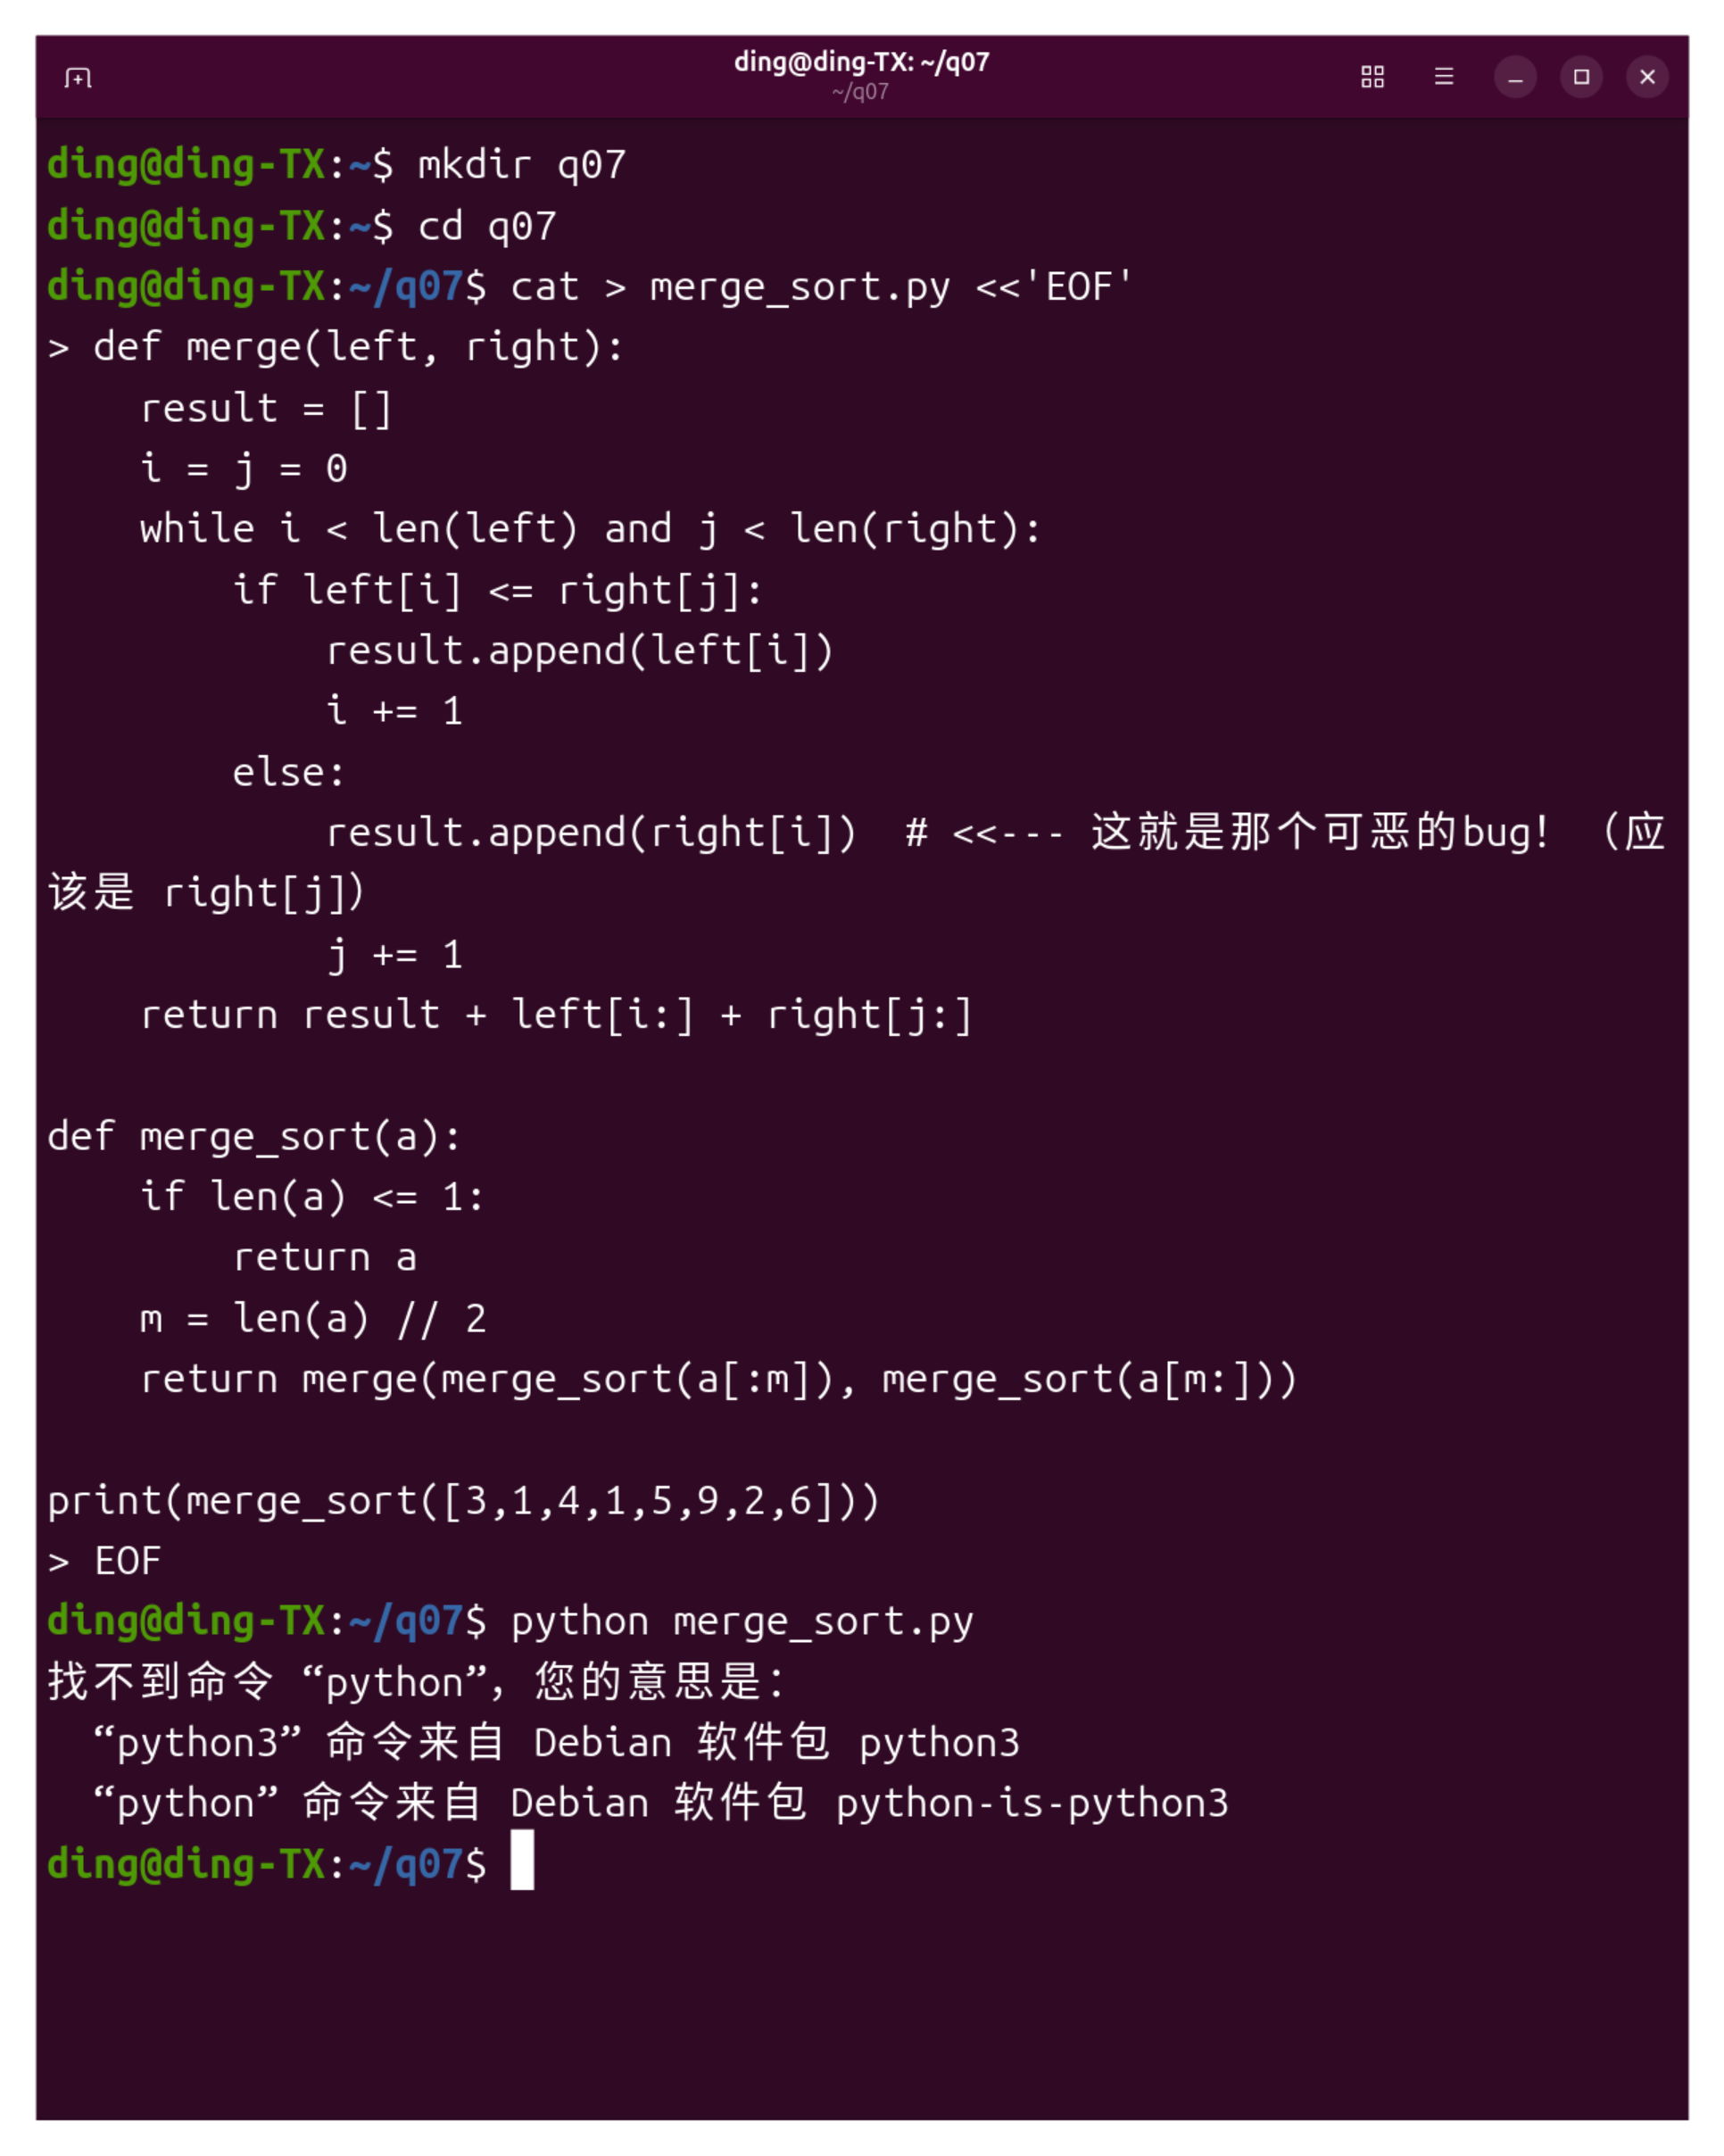
\includegraphics[width=0.9\textwidth]{q07_create_bug.png}
\caption{第7题步骤1：创建含缺陷的 merge\_sort.py}
\end{figure}

\textbf{步骤2：使用调试器定位缺陷。} 在 VS Code 中为 \texttt{merge} 设置断点，使用调试器（debugpy）单步执行，监视 \texttt{i}、\texttt{j}、\texttt{left}、\texttt{right}、\texttt{result} 的实时值。

\begin{figure}[H]
\centering
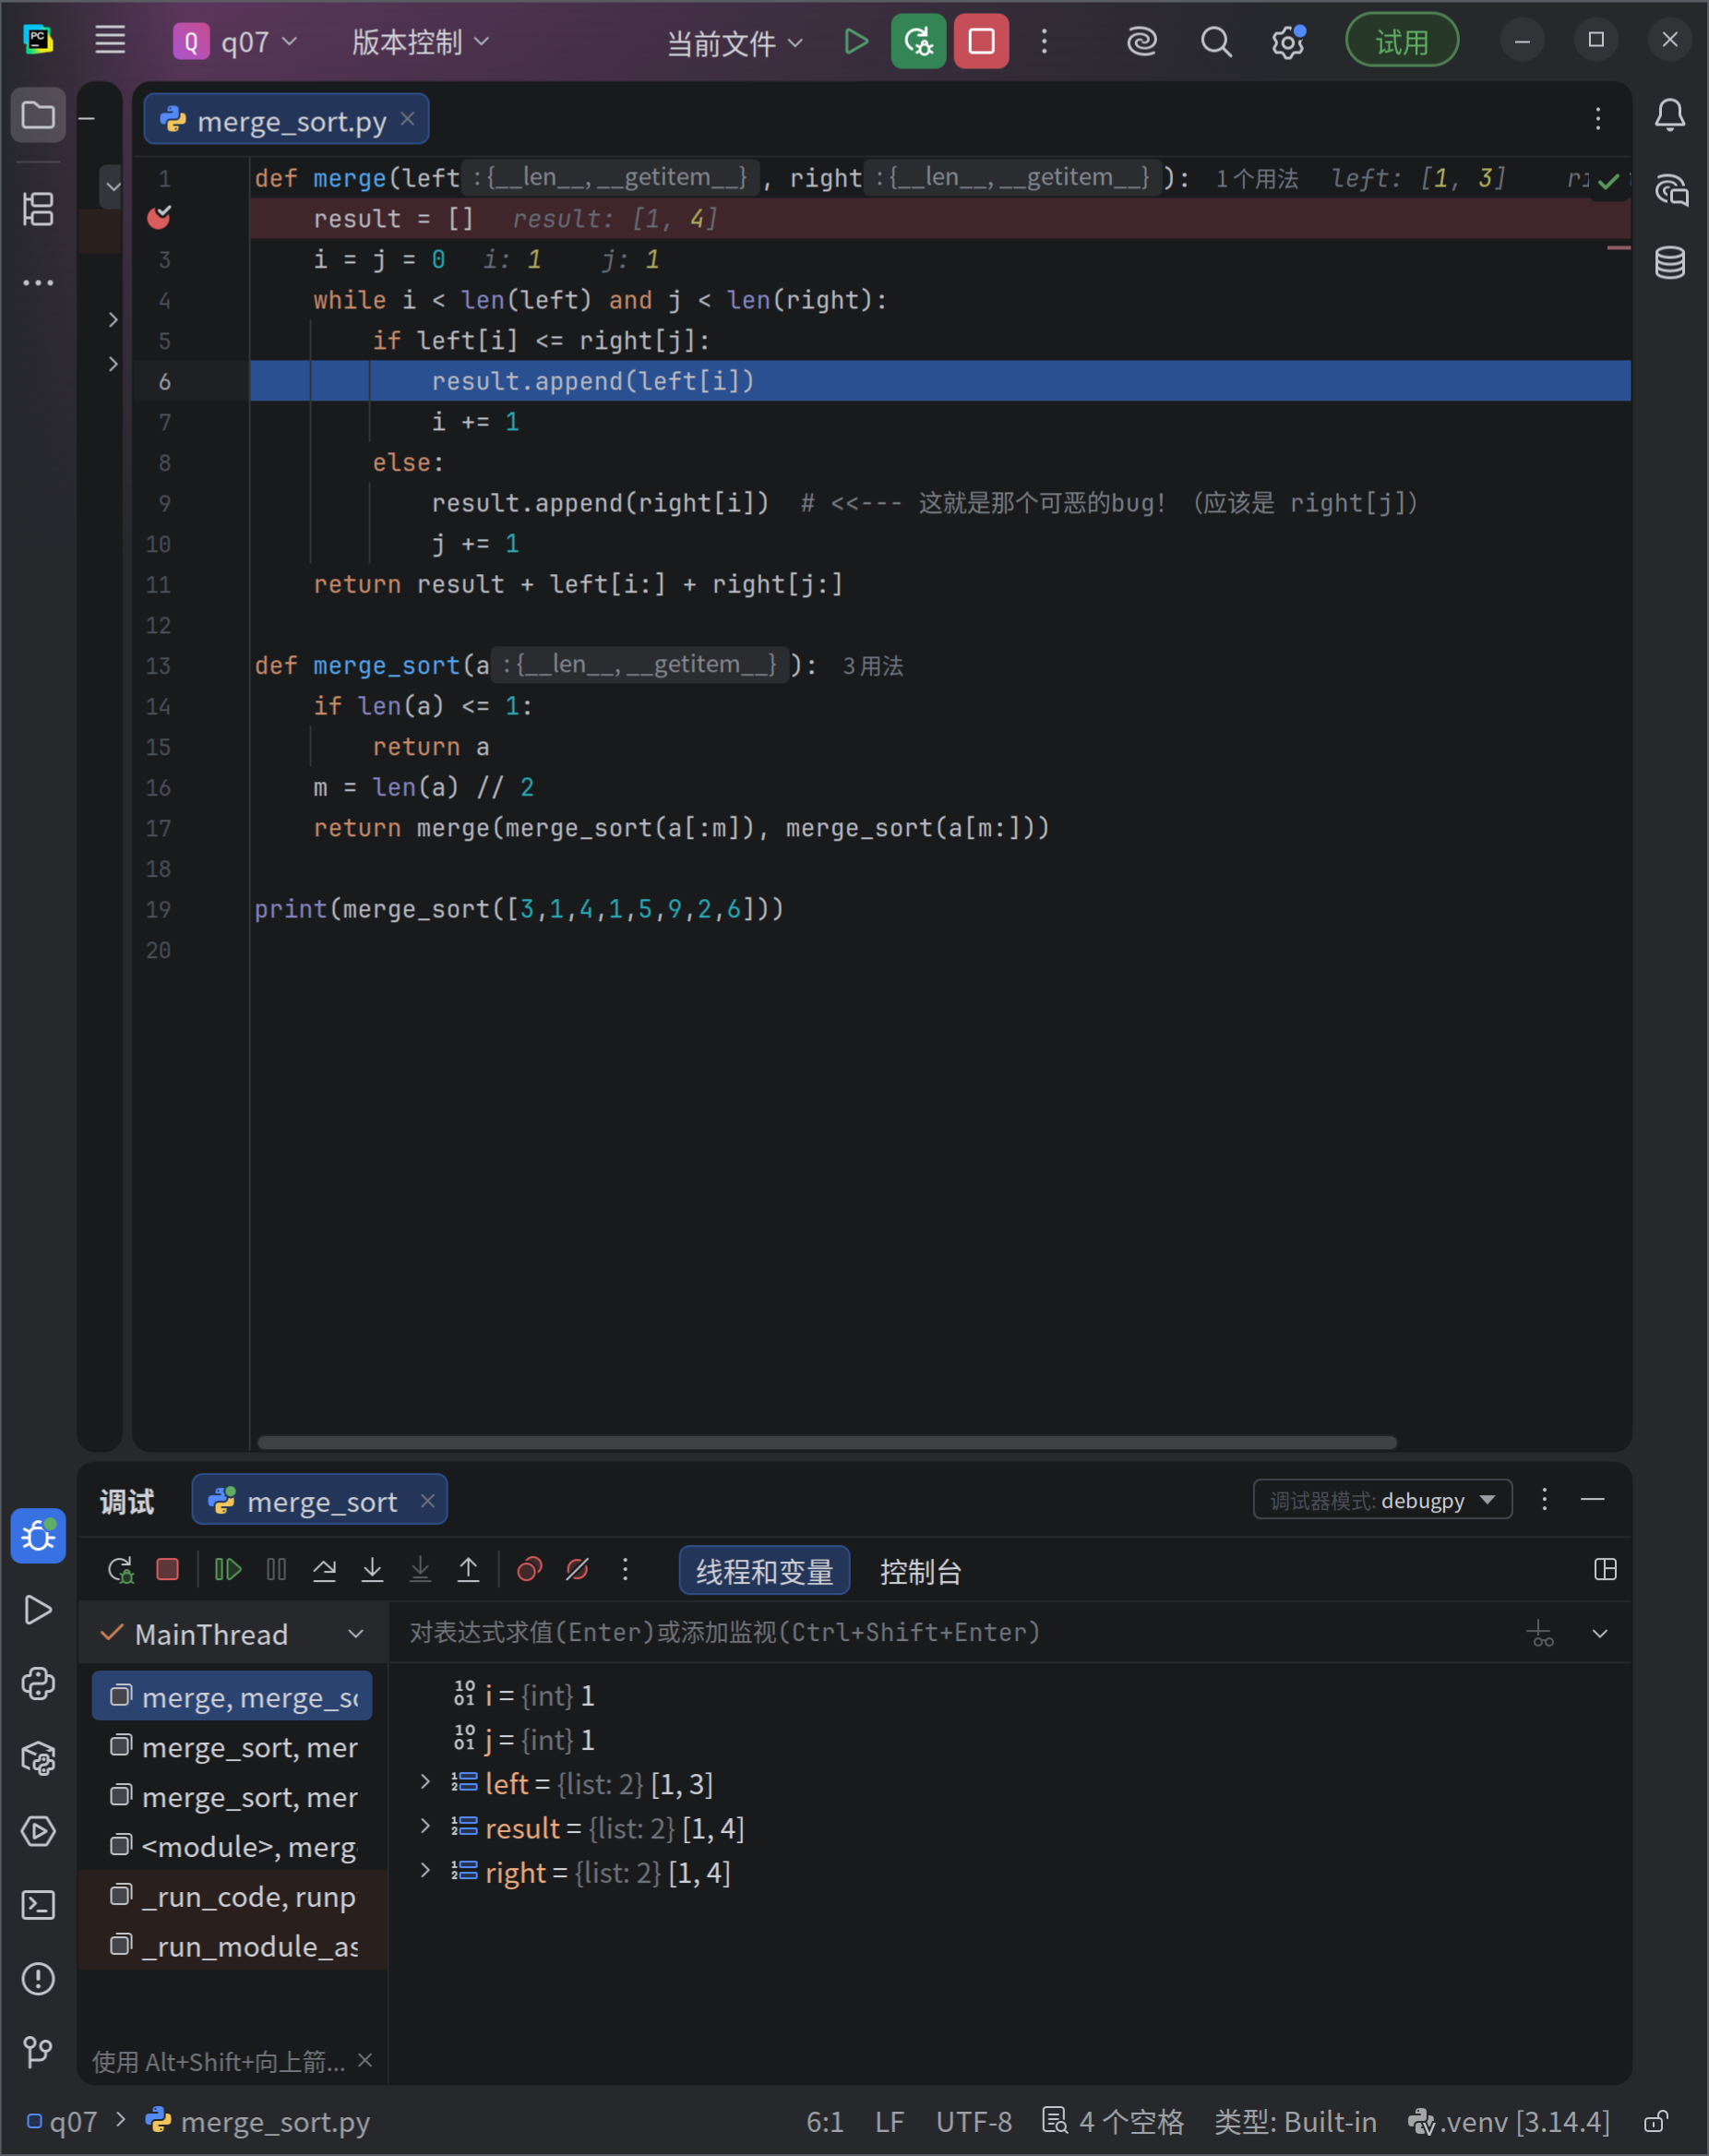
\includegraphics[width=0.9\textwidth]{q07_debug.png}
\caption{第7题步骤2：断点调试观察变量}
\end{figure}

调试中发现：当 \texttt{left=[1,3]}、\texttt{right=[1,4]}、\texttt{i=1}、\texttt{j=1} 时，\texttt{else} 分支执行 \texttt{result.append(right[i])}，用另一列表的下标 \texttt{i} 去索引 \texttt{right}，定位到索引错误——本应取 \texttt{right[j]}。

\textbf{步骤3：最小修复并验证。} 将 \texttt{right[i]} 改为 \texttt{right[j]}，重新运行，输出正确结果 \texttt{[1, 1, 2, 3, 4, 5, 6, 9]}，退出码 0。

\begin{figure}[H]
\centering
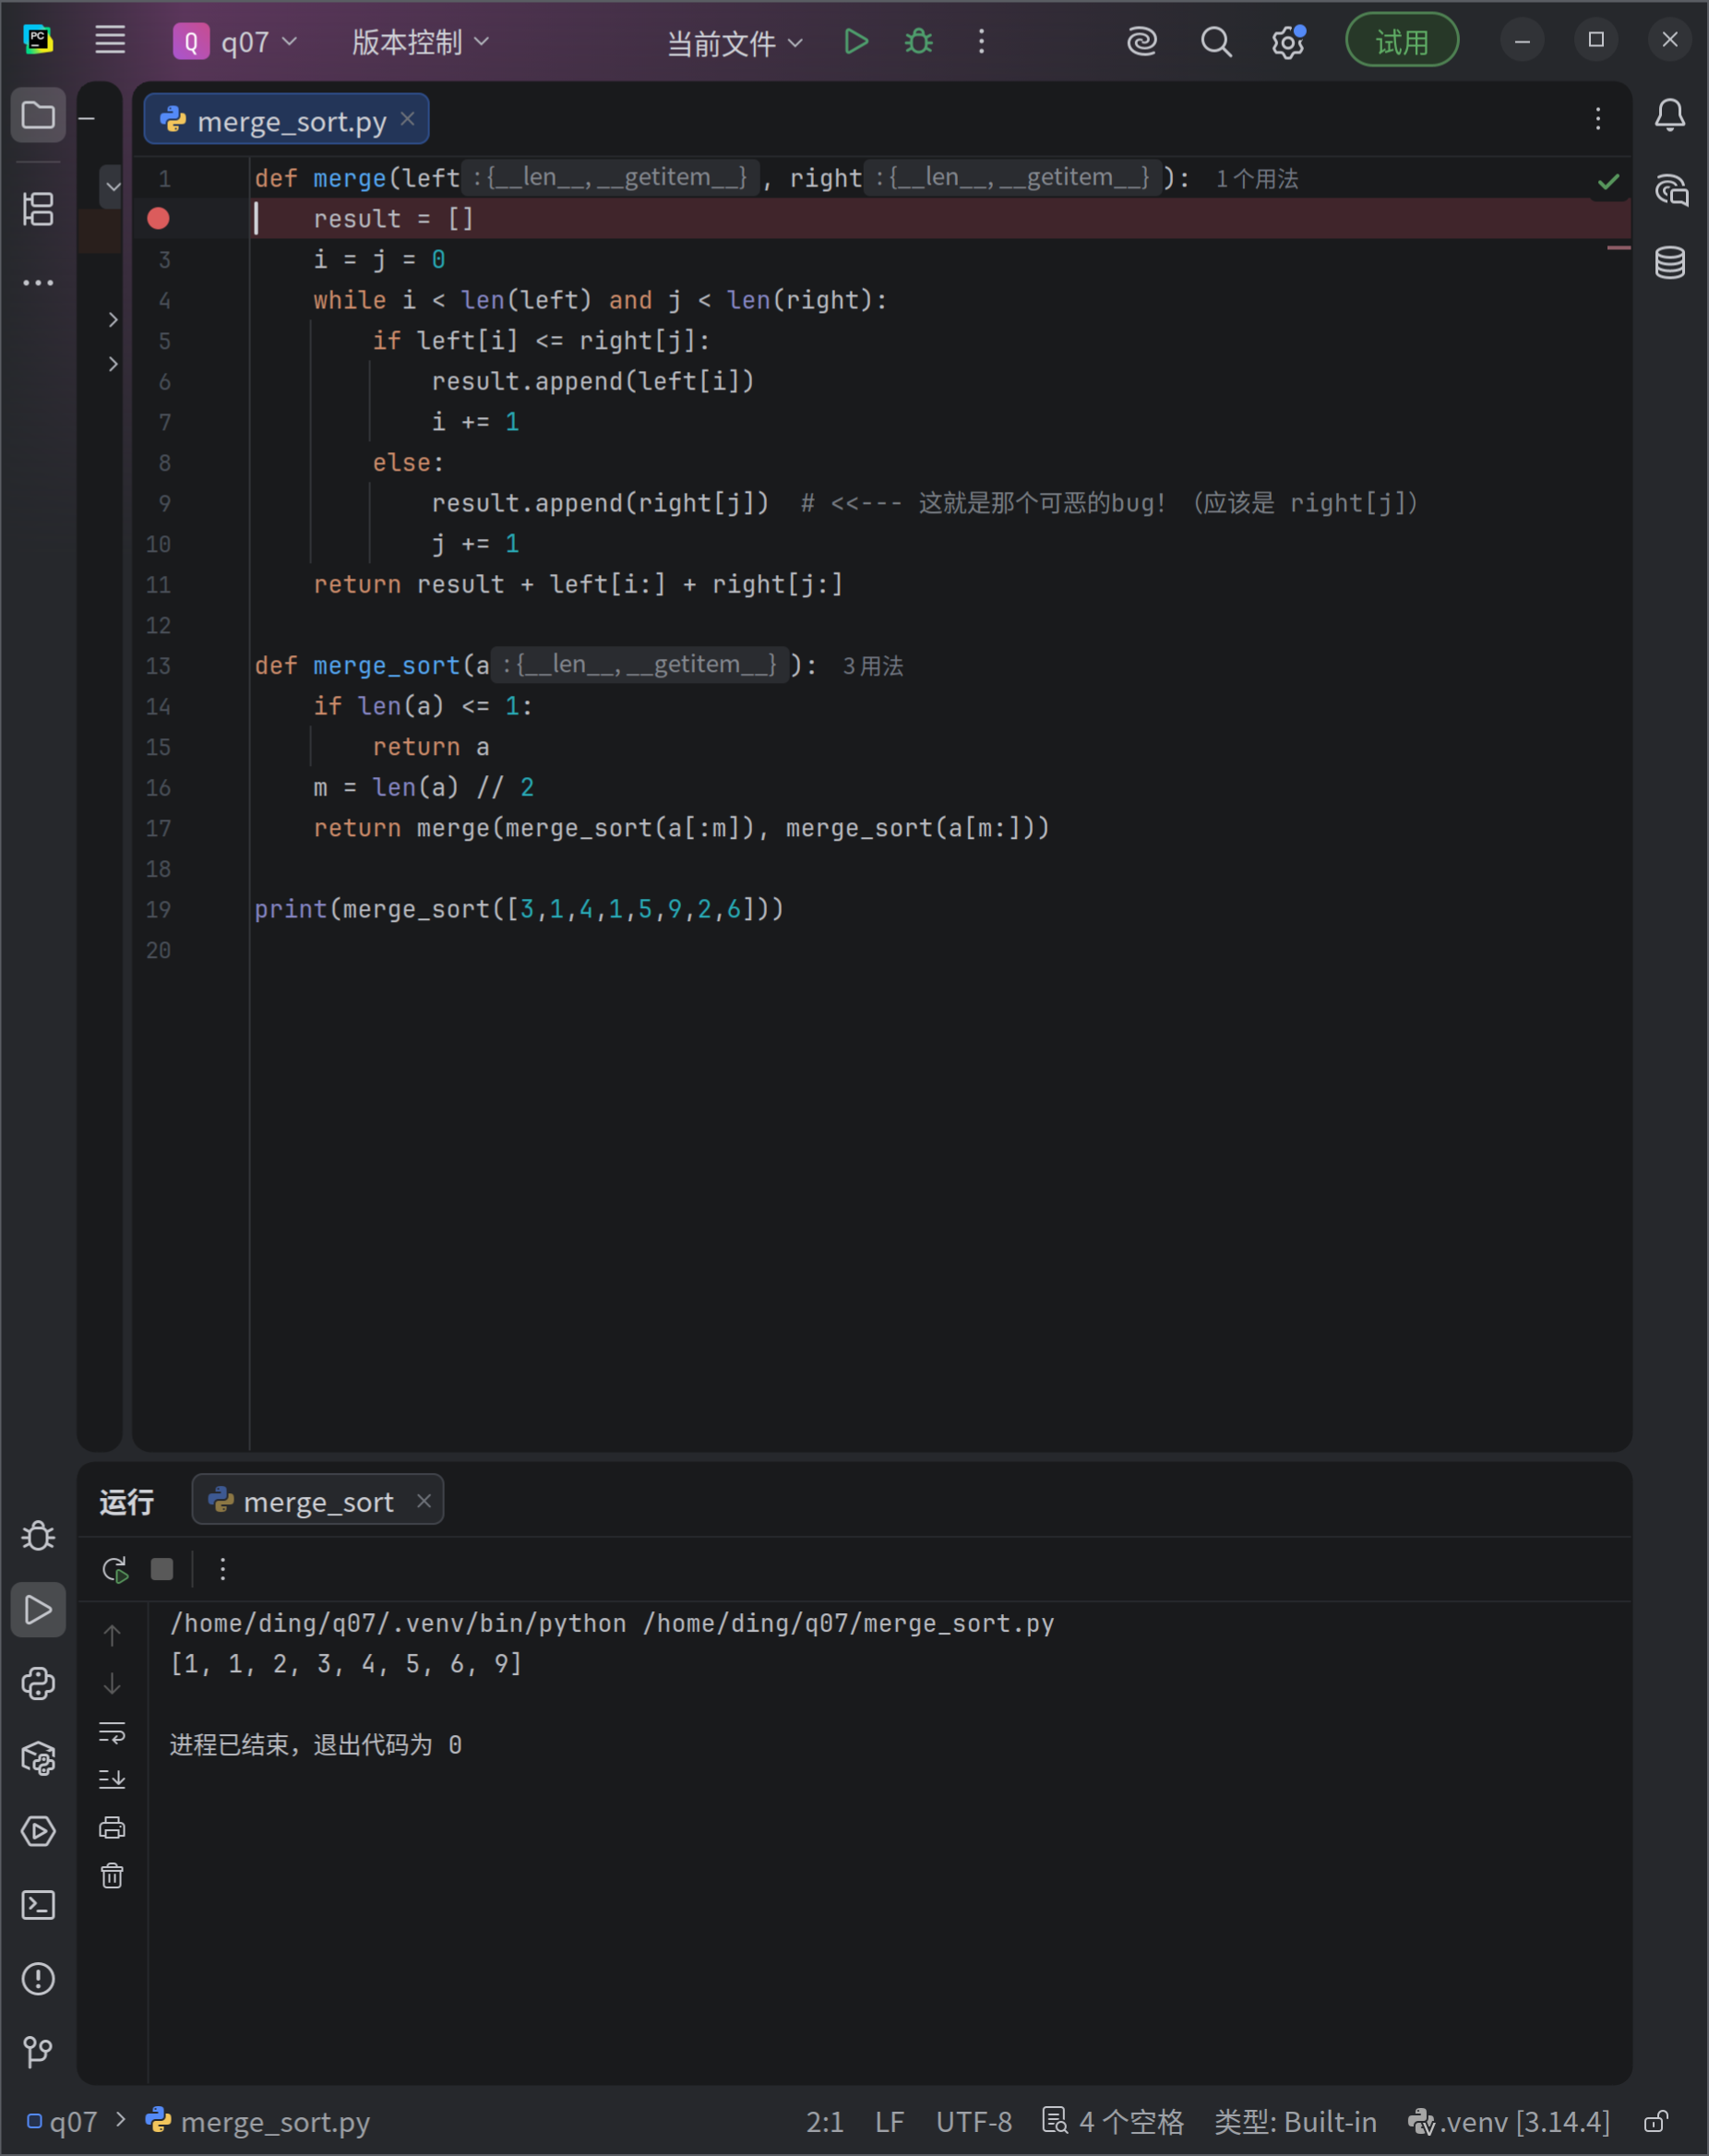
\includegraphics[width=0.9\textwidth]{q07_fixed_run.png}
\caption{第7题步骤3：修复后运行输出正确排序结果}
\end{figure}

\textbf{步骤4：pytest 单元测试。} 新建 \texttt{test\_merge\_sort.py}，按题目要求增加两个测试：给定输入和含重复元素的列表。

\begin{lstlisting}[language=Python]
from merge_sort import merge_sort

def test_merge_sort_given_input():
    # 给定输入
    assert merge_sort([3, 1, 4, 1, 5, 9, 2, 6]) == [1, 1, 2, 3, 4, 5, 6, 9]

def test_merge_sort_with_duplicates():
    # 含重复元素
    assert merge_sort([5, 2, 8, 2, 9, 1, 5, 5]) == [1, 2, 2, 5, 5, 5, 8, 9]
\end{lstlisting}

执行 \texttt{pytest}，收集到 2 个测试用例，全部通过：

\begin{verbatim}
test_merge_sort.py::test_merge_sort_given_input PASSED    [ 50%]
test_merge_sort.py::test_merge_sort_with_duplicates PASSED [100%]
============================== 2 passed in 0.22s ===============================
\end{verbatim}

\subsubsection{关键技术点}

\begin{enumerate}
    \item \textbf{断点调试}：在可疑分支设置断点、单步跟踪，比反复打印更能直观定位状态错误。
    \item \textbf{变量监视}：调试面板实时显示 \texttt{i}/\texttt{j}/\texttt{left}/\texttt{right}/\texttt{result}，能立刻发现下标错位。
    \item \textbf{最小修复}：只修改出错的一行，不重写算法，符合“最小改动”原则。
    \item \textbf{pytest 回归}：以 \texttt{test\_} 前缀自动收集测试函数，两个用例覆盖给定输入与含重复元素场景，防止修复引入回归。
\end{enumerate}

% ============================================================
\section{进度说明}
% ============================================================

本次实验共 4 题，目前已完成前 3 题（第5、6、7题），第7题的缺陷调试、修复与 pytest 单元测试均已补齐。第8题（先测量，再优化慢速词频程序）尚未完成，待完成后再补充到本报告中。

\end{document}
